%!TEX encoding = UTF-8 Unicode
%!TEX TS-program = xelatex
%% This template licensed under CC-BY-NC-SA by Koenraad De Smedt
\documentclass[letterpaper,12pt]{article}
\usepackage[margin=1in]{geometry}
\usepackage{graphicx}

% \usepackage{fontspec,xltxtra,polyglossia,titling,graphicx}
% \usepackage{verbatim,gb4e,synttree,multicol} % choose or add what you need
\usepackage[colorlinks,urlcolor=blue,citecolor=blue,linkcolor=blue]{hyperref}
%\setmainfont[Mapping=tex-text]{Times New Roman} % or another similar font
%\setdefaultlanguage{english}

\usepackage{subcaption}
\usepackage{fancyvrb}
\usepackage{natbib}
\usepackage{tabularx}
\bibliographystyle{chicago}

\title{“Real-Time 3D Reconstruction from ROV Camera Arrays of Opportunity”}

\begin{document}
\begin{center} 

\vfill

{\large NOAA Office of Exploration and Research (OER)\\
Award \#NA160AR0110195}

\vspace{1em}

\textbf{\Large “Real-Time 3D Reconstruction from ROV Camera Arrays of Opportunity”}

\vfill

PI:   Aaron Marburg \\
University of Washington  \\
Applied Physics Laboratory \\
Seattle, WA \\
amarburg@apl.washington.edu \\
206-685-8461

\vfill

Funding:  \$105,720

Period of Performance:  9/1/2016 – 8/30/2018

Progress Report for Period:   9/1/2016 - 8/30/2018 \\
\textbf{Final Report}

\vfill 

%
\end{center} \clearpage


\subsection*{Abstract} 
1-paragraph description of final report

\section{Summary}

\subsection{Purpose of Project}

This project examined the applicability of photogrammetric 3D reconstruction for ROV-based exploration.   Photogrammetric or image-based 3D reconstruction is the process of using large numbers of still images (or frames from video) to produce a 3D model of the scene shown in the images.   In its simplest form, photogrammetric reconstruction requires only images as an input, estimating both scene structure and camera positions/trajectory as an outcome of the optimization process.   To form this optimization, the reconstruction uses image-matching techniques to extract points in two or more input images which correspond to the same world point.   Each of these inter-image correspondences forms a geometric constraint.   Given sufficient numbers of these constraints, a bulk non-linear optimization, typically referred to as \textit{bundle adjustment}, can be solved for both the 3D arrangement of the world points and for the camera positions.   The general field of reconstruction tools can then be further divided into post-processed and real-time operations.   The former focuses on reconstruction from sets of images after collection.  As such, the sets of images are often hand-selected or hand-curated from a larger original data set, processing time or performance is less of a concern, and the processing does  not necessarily know or take advantage of the order in which images are taken.   As the reconstruction software has access to the full sequence of images, it actively seeks image correspondences across all pairs and forms a more dense network of correspondences, and can generally be considered ``optimal'' for a given set of input images.   However, post-processed results may take hours or days to produce and are not generally available during data collection.

Alternatively, real-time reconstruction algorithms are designed for processing data as it streams in, either as video or a sequence of images.   In contrast to post-processed, real-time algorithms are heavily tuned for performance and in many cases sacrifice the resolution, is not the accuracy, of the resulting reconstruction to process incoming data in a timely manner.   Generally, real-time algorithms also privilege matches between the current image and recent images over more temporally distant images, and as a broad statement, then, tend to produce less complete inter-image correspondence sets and thus less optimal final products.   In exchange for this reduced data quality, real-time algorithms offer the possibility of ``growing'' a 3D reconstruction immediately as data arrives from the primary sensor.    Strictly from a data point of view, this immediate feedback might be used to identify and remedy data quality issues which might impact later post-processed reconstructions.  For example, a real-time reconstruction would show regions in a scene which had not yet been imaged as ``holes'' or data voids, which could then be explicitly imaged as part of the ongoing data collection.   With the long processing cycle of post-processed reconstruction, this data gap might not be noticed until after it is too late to remedy.  In the future, the live reconstruction could also play a part in on-line mission planning and visualization, for example, a reconstruction could provide a 3D map of a vehicle's trajectory and current location within a scene far better than the singular view through the ROV main camera.  This could assist in scene-relative navigation (e.g., ``return to that point which is behind you and to the left'').    Taking an even longer view, 3D reconstruction is one valuable technique for generating machine format scene information as an input to robotic autonomy or semi-autonomy for ROV-like vehicles.  

As high-quality imaging data is relatively simple to acquire, photogrammetric reconstruction has become a popular technology for ``3D scanning'' of objects and scenes.  However, due to its computational complexity and sensitivity to certain conditions in image acquisition, it has excelled in certain niches (large scale outdoor acquisition) whereas other, more specialized technologies (e.g., structured light sensors, LiDAR) are more prevalent in other applications.    

The broad question addressed within this project is the applicability and usefulness of 3D reconstruction to ROV-based exploration, and particularly as an value-added product which does not drive specific mission behaviors for its acquisition, but which is generated organically as part of standard ROV operating procedures.  This project, then, addressed three main questions:

\begin{itemize}
    \item First, are segments of the archival D2 video suitable for post-processed reconstruction?   Are there structural or operational impediments to performing 3D reconstruction with the D2 video?   Post-processed reconstruction may be a valuable added product from particular ROV dives, particularly when exploring sites where the geometry of the site at a $\sim 1-10$ m scale is of particular interest.  As reflected in the D2 video analyzed within this project, this includes many archaeological explorations,  hydrothermal vent structures, and larger coral reef communities.   As shown in one of the dives (EX1605L3\_DIVE04\_20160621), reconstruction can also be useful for visualizing topography over short transects although the lack of ground truth information makes reconstruction \textit{without} explicit provision in the mission planning less useful.
    
    \item Second, having shown that a segment of video can be reconstructed under controlled post-processed conditions, can those same segments be reconstructed using a real-time algorithm?   This question occupies the bulk of this project for two reasons:  first, as discussed previously, real-time reconstruction is inherently a technically more challenging endeavour than post-processed reconstruction.  Second, whereas the post-processed reconstruction uses a commericial off-the-shelf application, there are no commercial generalizeable real-time reconstruction software packages.  Instead, most real-time software remains in the academic realm, and requires significant effort to understand, use, and modify for the specific application.  

    \item Finally, having processed D2 video from a variety of missions, is the collected video suitable for 3D reconstruction?  This is a multi-faceted question.  First, is the video data itself suitable for reconstruction?  Given the overall image quality of the main HD camera, this is assumed to be true.  Second, do the procedures for recording and storing archival ROV video enable reconstruction.   Finally, and most importantly, are the standard operating procedures for the ROV \& camera amenable to reconstruction when reconstruction is not the explicit mission goal for a dive or segment of a dive.  During a dive, the set of decisions which dictate the motion of the ROV and camera encompass a large number of stakeholder needs and constraints, ranging from the capabilities and physical safety of the ROV, through to the science goals of the staff onboard the \textit{Okeanos Explorere} and on telepresence.  In an ideal world, reconstructions could be produced without impacting this set of constraints; or as a compromise, a well-defined set of standard operating procedures for collecting data suitable for reconstruction could be established.  
    
\end{itemize}

% \subsubsection*{Describe issue that was addressed}

% \subsubsection*{Describe and list the project objectives}

\subsection{Approach}
\subsubsection*{Describe the work that was performed}

Project work fell into three major tasks.  First was acquisition of the archival D2 video and development of tools for accessing and extracting useful subsets of the video.  This development also included exploration of the ~32 hours of video to identify short subsets suitable for reconstruction.   Second was the processing of those subsets using Agisoft Photoscan, a commercial 3D reconstruction package.   Third was the processing of those subsets using LSD-SLAM a realtime reconstruction package.  Whereas Photoscan could be used out-of-the-box for the second task, the third required significant development of the LSD-SLAM package to produce a robust realtime reconstruction solution.  

Input video was provided by the NOAA data archive.  In collaboration with archivists, four D2 dives from the NOAA expedition \textit{EX1605: Deepwater Exploration of the Marianas} were identified as having regions which might be suitable for reconstruction:

\begin{itemize}
    \item \textbf{Leg 1, Dive 11: New Vent Field} (\textit{EX1605L1\_DIVE11}).   An approx 6h30m dive exploring an area previously mapped by the Sentry AUV and believed to contain multiple previously unexplored hydrothermal vents. This dive was selected as hydrothermal vent structures provide a dramatic 3D shape which might be explored in more detail through reconstruction.    This video would be challenging due to the high level of motion around a vent due to schlieren, macrofauna, and particulates/precipitates/smoke.
    
    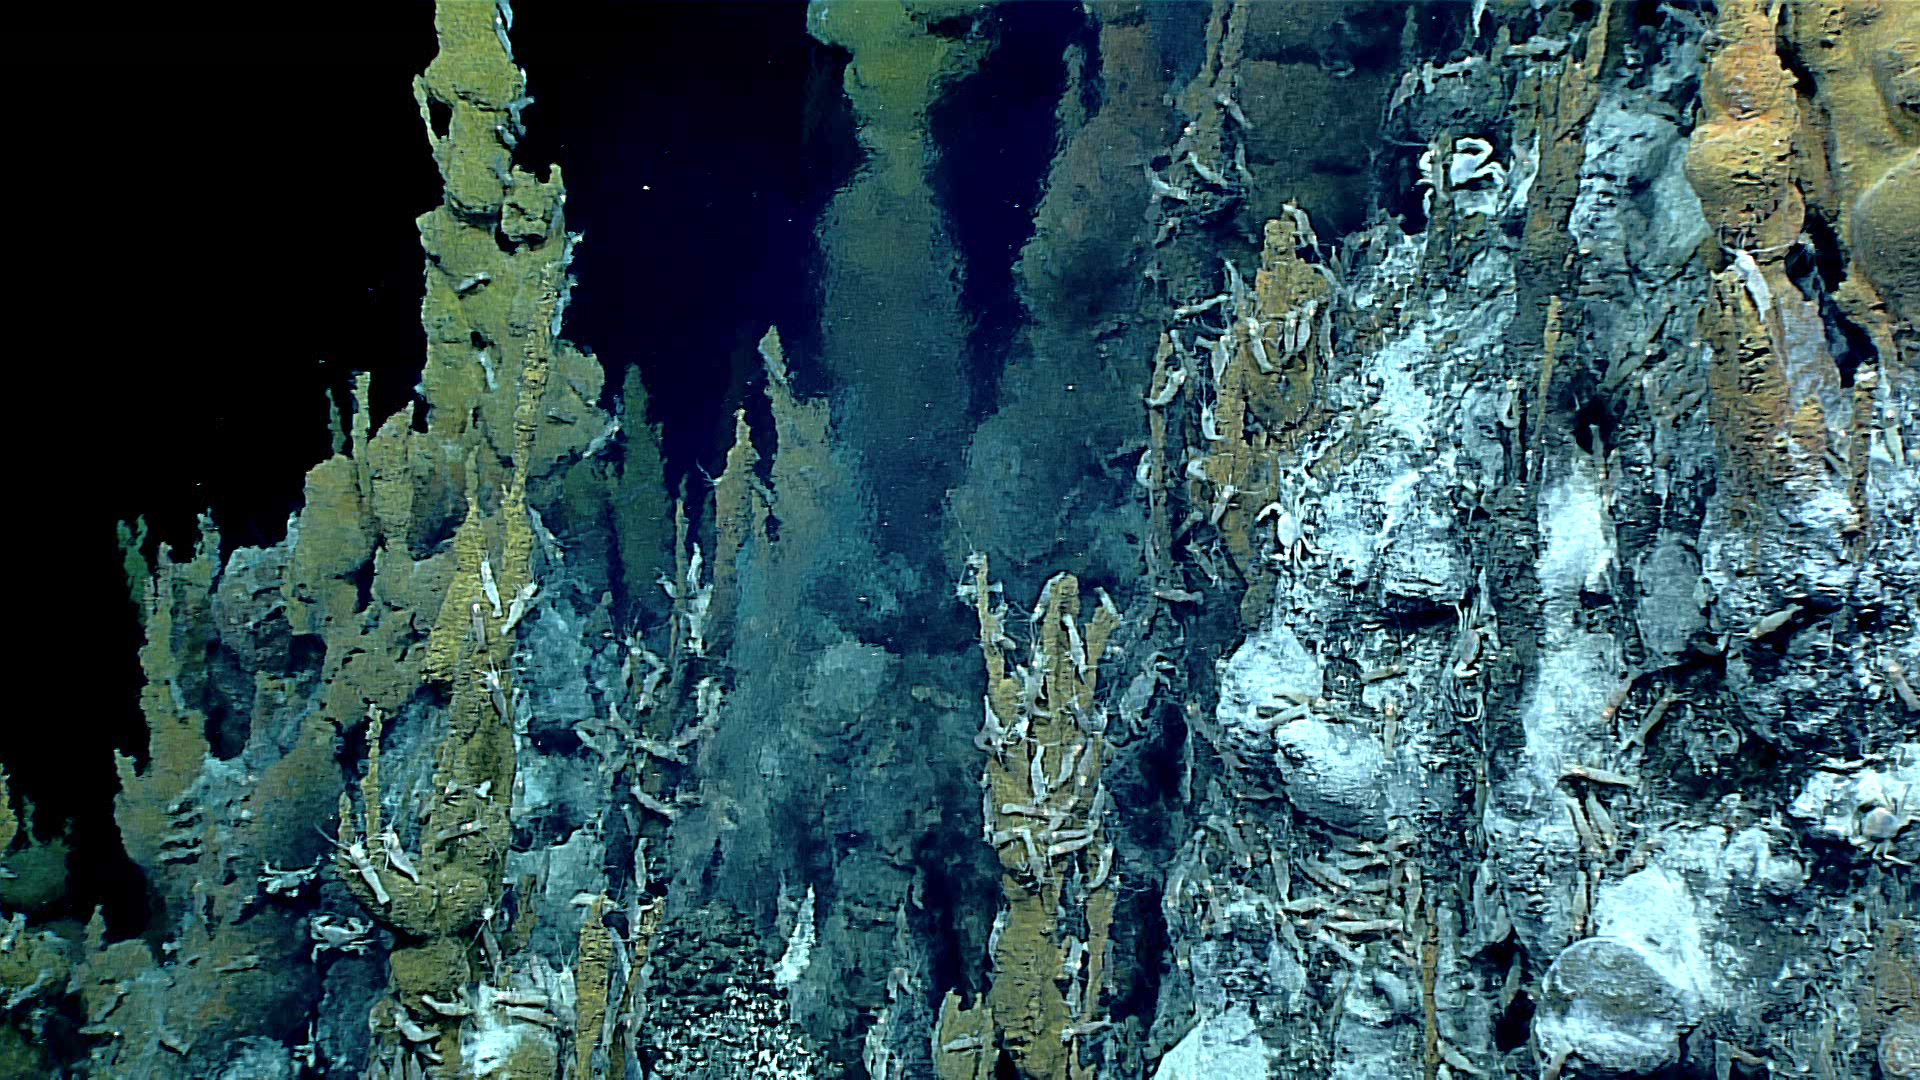
\includegraphics[width=0.5\textwidth]{images/EX1605L1_DIVE11_highlight.jpg}
    
    \item \textbf{Leg 3, Dive 4: Hadal Ridge} (\textit{EX1605L3\_DIVE4}).  Approximately 2h51m of this 10h dive was spent on the bottom, transecting up-slope through a region of fine sediment with some rocky outcroppings.  This video was selected to evaluate the potential of using photogrammetry to estimate vehicle trajectory during long transects.
    
    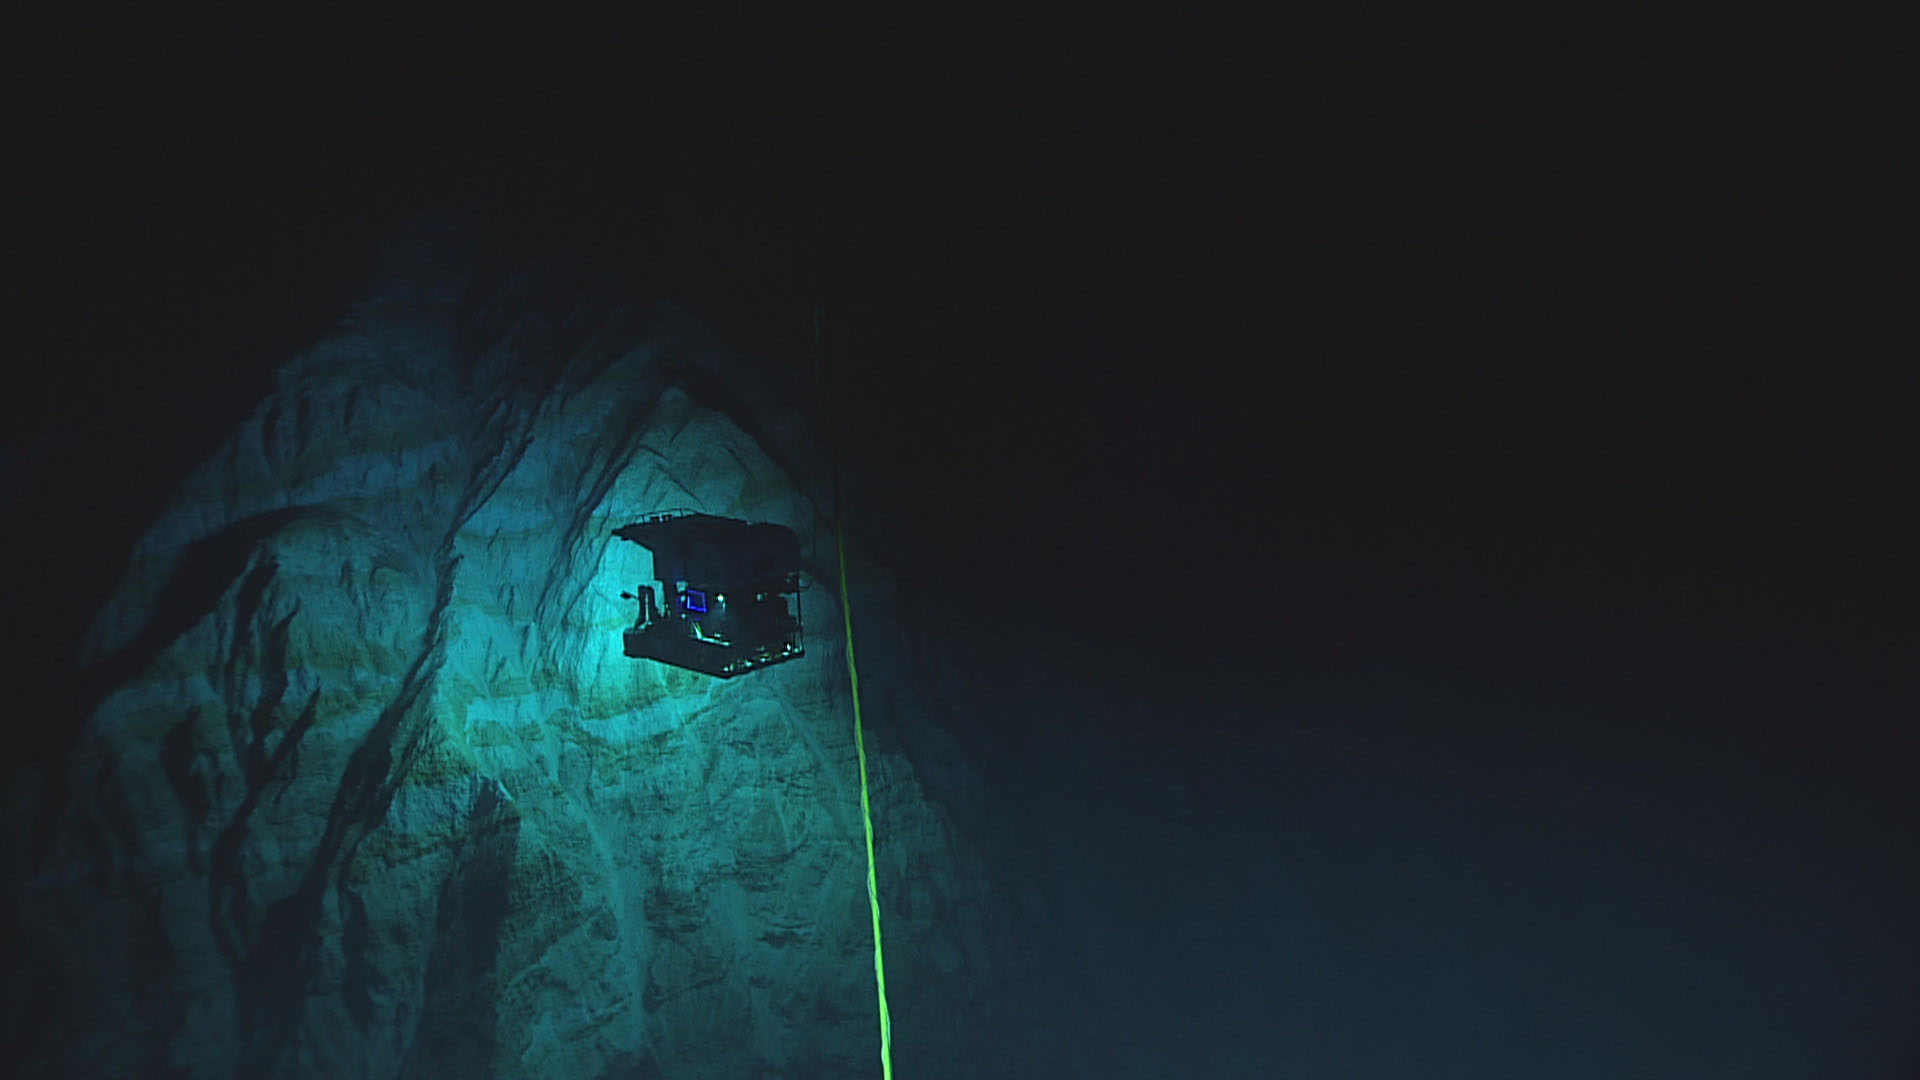
\includegraphics[width=0.5\textwidth]{images/EX1605L3_DIVE4_highlight.jpg}
    
    \item \textbf{Leg 3, Dive 7: Chamorro Seamount} (\textit{EX1605L3\_DIVE7}).  Approximately 7h on the bottom in a rocky region including several smaller hydrothermal vents.    This video was selected to evaluate reconstruction of smaller rocker outcropping and vents, and also for mapping of transects over rocky terrain.
    
    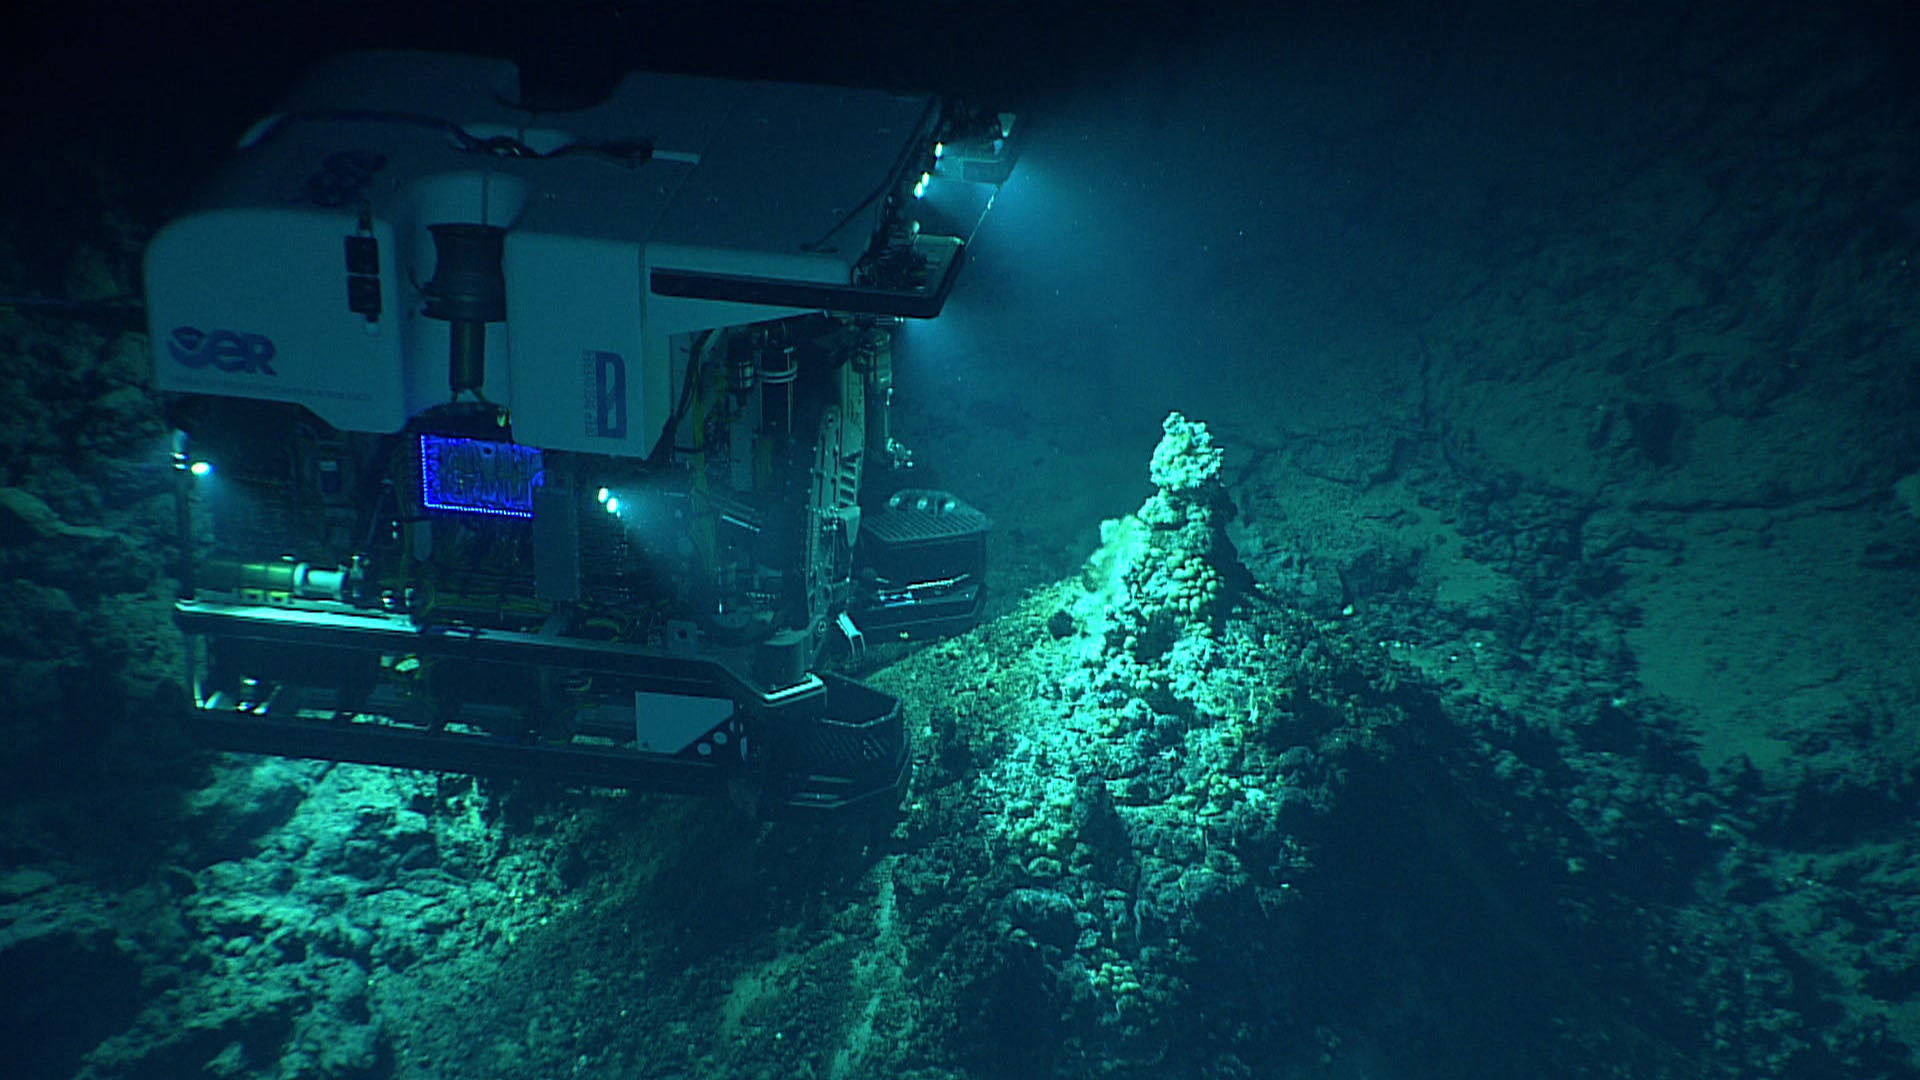
\includegraphics[width=0.5\textwidth]{images/EX1605L3_DIVE7_highlight.jpg}
    
    \item \textbf{Leg 3, Dive 22: Romeo and Juliet} (\textit{EX1605L3\_DIVE22}).  This dive explores two sonar anomalies in the Saipan channel believed to be crashed B-29 aircraft from World War Two.  This video was selected to demonstrate reconstruction of archaeological artifacts.
    
    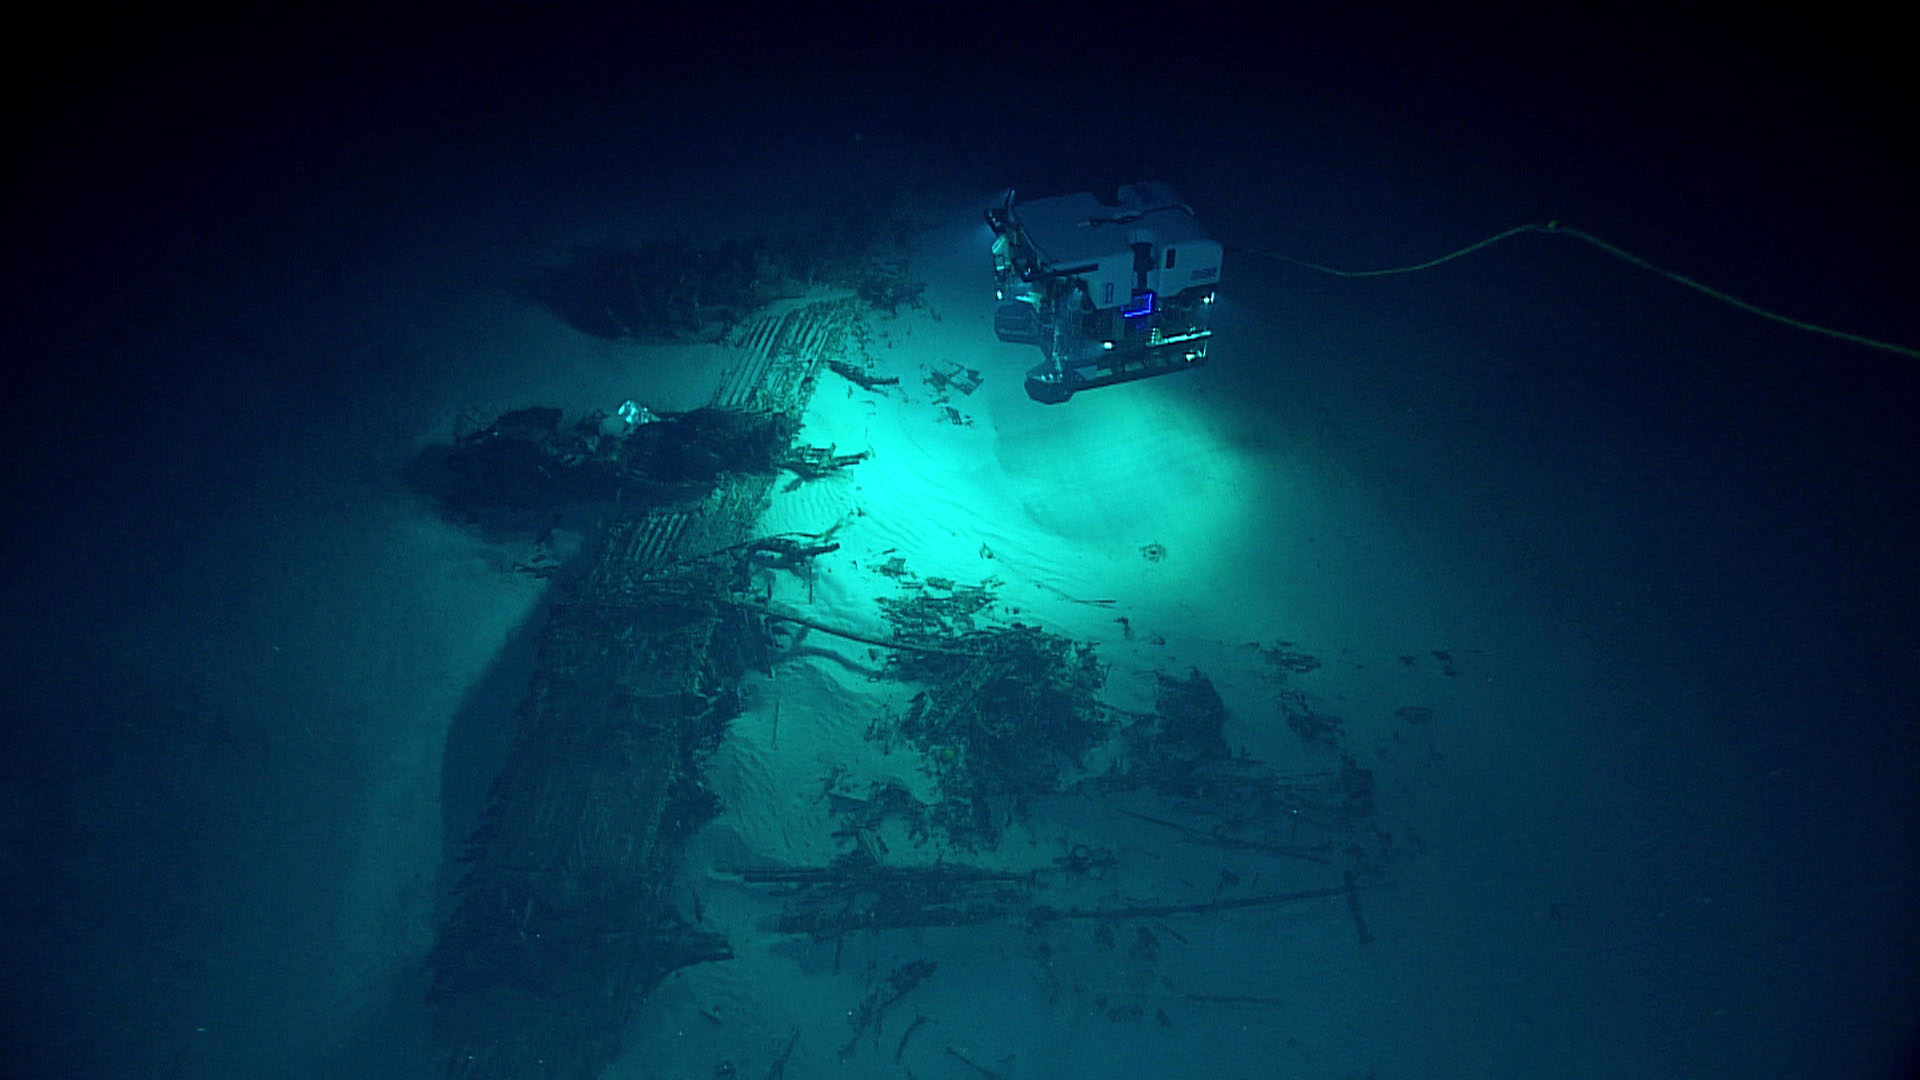
\includegraphics[width=0.5\textwidth]{images/EX1605L3_DIVE22_highlight.jpg}
    
\end{itemize}

Approx 4.2TB of video was delivered by external hard drive from the NOAA data archive.  All video products for all four dives were provided, including the full QuickTime/ProRes-encoded stream from the main science camera, as well as selected video subsets from both the main science camera and supplemental cameras, including the brow cameras on D2, and the \textit{Seirios} camera.   The latter supplemental data sets were not continuous through the dive and were provided at each camera's resolution, typically standard definition (SD).  

Initial work focused on the full-resolution, full-mission-length HD main science camera video.  This video was delivered as a sequence of 5-minute-long Quicktime movies encoded with the ProRes video codec, covering the entire dive from surface to surface.    As an example, Leg 3 Dive 7 is recorded as spanning 8h17m from 20:19:04 UTC to 05:19:18 UTC the subsequent day.  It is provided as 105 videos timestamped from 20:15:00 UTC to 04:55:00 UTC, totalling 521GB of video. 

\subsubsection{Video Indexing and Annotation}

For each video the initial step was to identify and isolate short, self-contained segments of each mission which might be suitable for reconstruction.   This effort leveraged previously-developed software tools for indexing and extracting individual frames from Quicktime/Prores files.  These tools were expanded to allow the aggregation of multiple sequential video files as a single entity, allowing time- and frame-based indexing from the start of the dive, rather than maintining bookkeeping across multiple discrete video files.  This technique was used extensively throughout the project.  As an example, a small utility was created which produces a thumbnail image approximately every minute through the length of a dive (figure \ref{img:thumbnails}), allowing quick scanning of an entire video file.

\begin{figure}
    \centering
    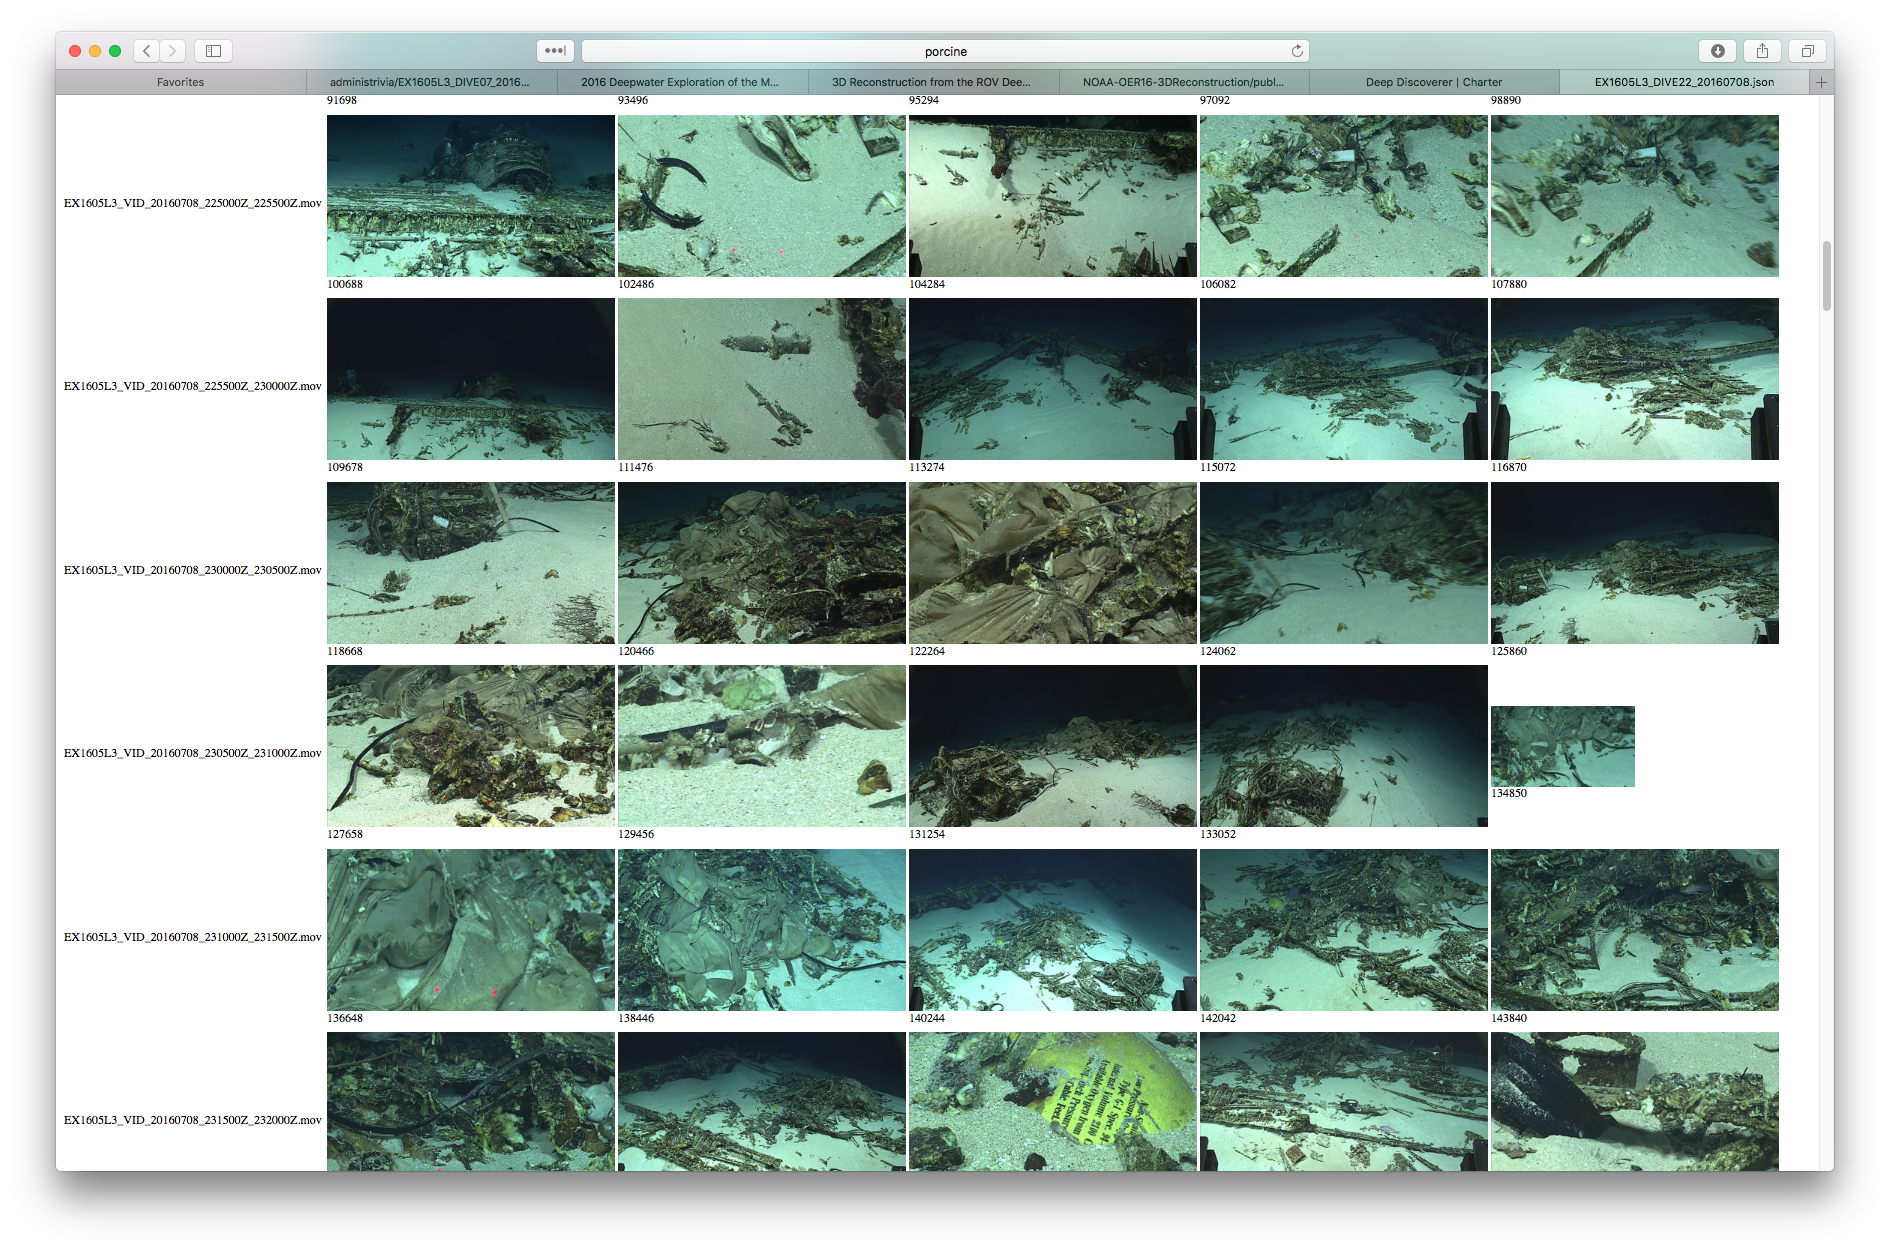
\includegraphics[width=0.9\textwidth]{images/thumbnailer_screenshot.png}
    \caption{Screenshot from video synopsis tools.   Constituent video files are shown in leftmost column.   One thumbnail image is drawn every minute of video.  Numbers under video give that frame's position within the dive, indexed from the beginning of the first video in the dive.}
    \label{img:thumbnails}
\end{figure}

This strategy was selected to allow documentable, repeatable delineation and extraction of subsets from a given video.  Using this tool, a small number of test subsets were identified.   Initial work quickly narrowed to just two dives: EX1605L3\_DIVE4 and EX1605L3\_DIVE22.  For each dive, an additional meta-data records was generated in JSON format.  The ``synopsis'' format:

\begin{Verbatim}[fonstize=\small]
{
  "Source": "$NOAA_DIR/EX1605L3/EX1605L3_DIVE22_20160708/Full/EX1605L3_DIVE22_20160708.json",
  "Chunks": {
    "descending": {
      "range": {  "start": 1  }
    },
    "approaching bottom": {
      "range": { "start": 38800 }
    },
    "approaching wing": {
      "range": { "start": 58800 }
    },
    "engine one": {
      "range": { "start": 63500 }
    },
    "landing gear": {
      "range": { "start": 71500 }
    },
    ...
\end{Verbatim}

allow definition of predefined ``regions'' or ``bookmarks'' within a video, for later access.  Both EX1605L3\_DIVE4 and EX1605L3\_DIVE22 were annotated in this manner.



\subsubsection{Post-Processed Reconstruction}

A segment from each video was selected for reconstruction using Agisoft Photoscan.   Based on the standard operating procedure of the ROV, these segments corresponded with periods of area exploration with the science camera in a zoomed-out state, and were bounded in both cases by the science camera moving to a full-zoom-in condition, examining an object at the behest of the science team.    

Within dive EX1605L3\_DIVE4, three periods of interest, labelled as ``hillside'', ``upslope'' and ``top\_of\_slope'' were examined.   ``Hillside'' starts with the ROV advancing towards a rocky slope (figure \ref{img:ex1605l3_dive4_hillside_start}).

\begin{figure}
    \centering
    \begin{subfigure}[b]{0.48\textwidth}
        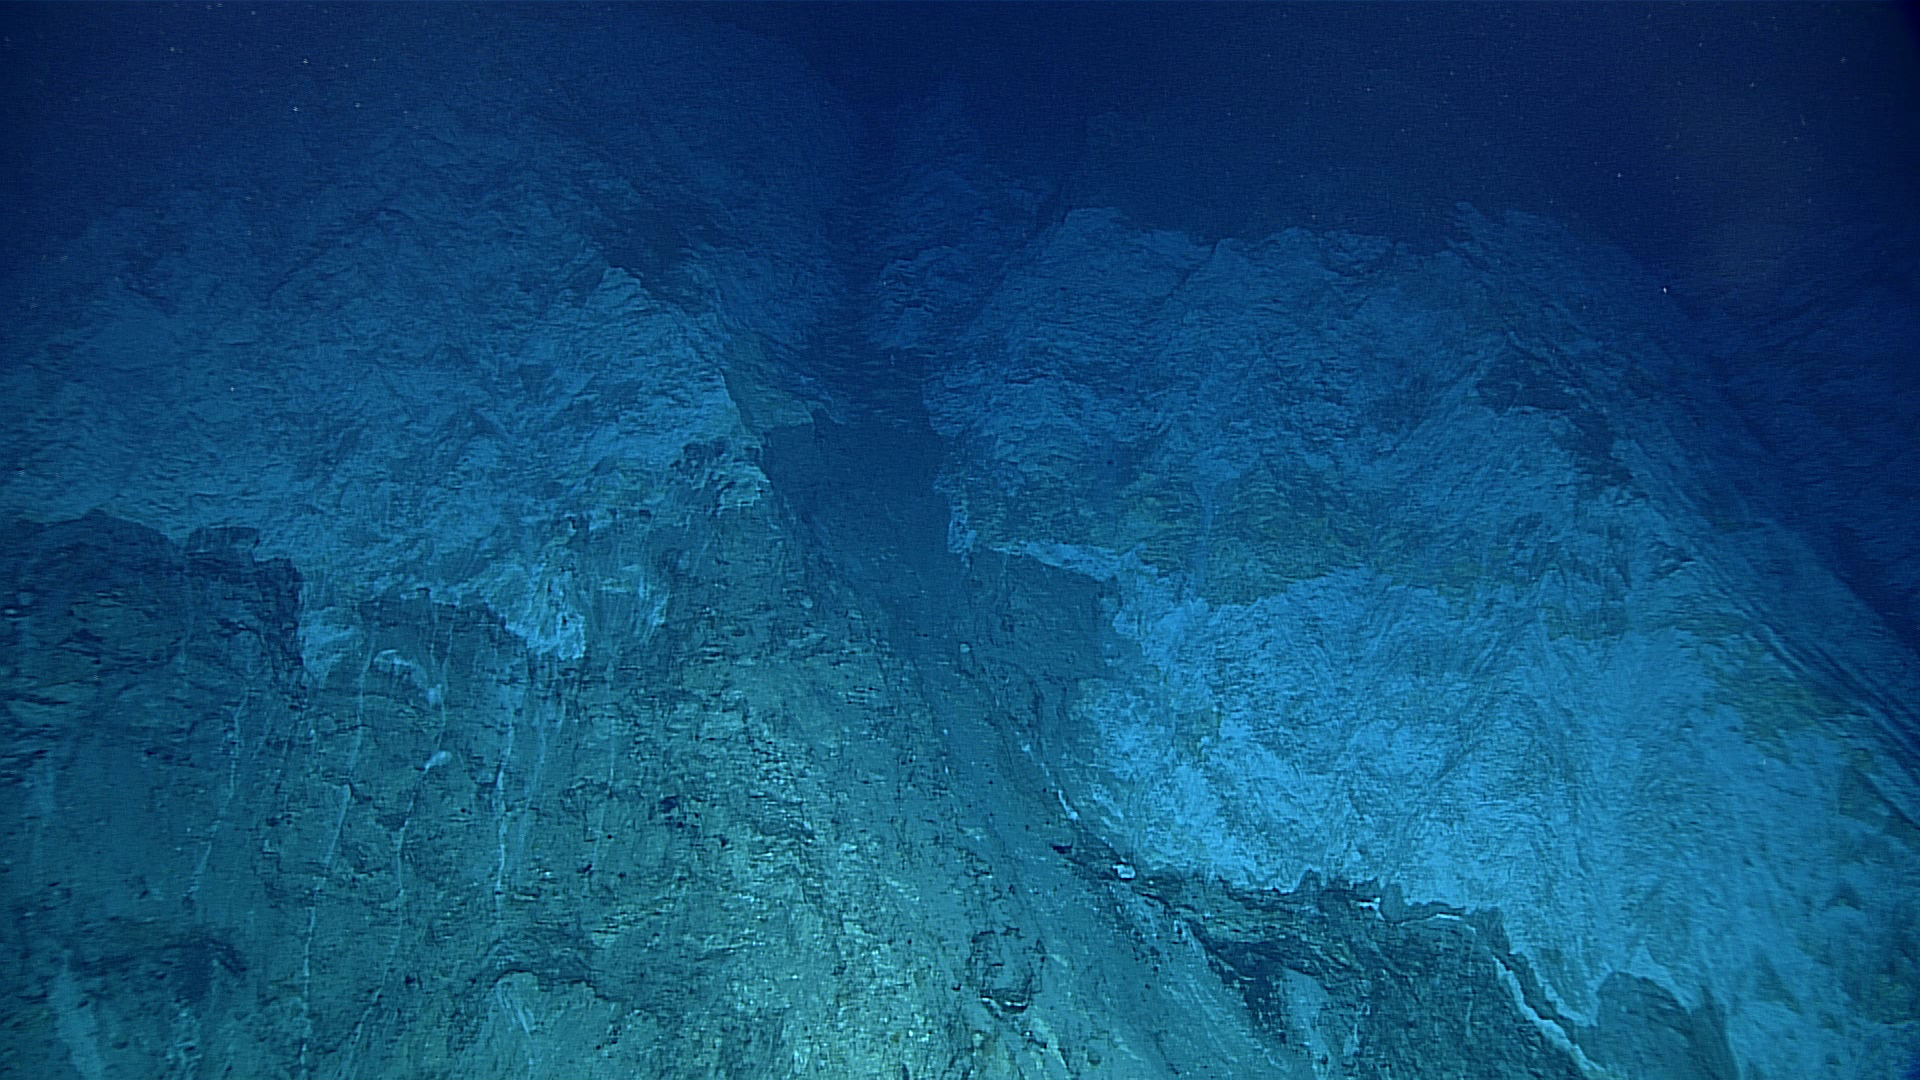
\includegraphics[width=\textwidth]{images/image_643000.png}
        \caption{First frame in reconstructed segment, frame 643000 within dive.}
        \label{fig:ex1605l3_dive4_hillside_begin}
    \end{subfigure}
    \begin{subfigure}[b]{0.48\textwidth}
        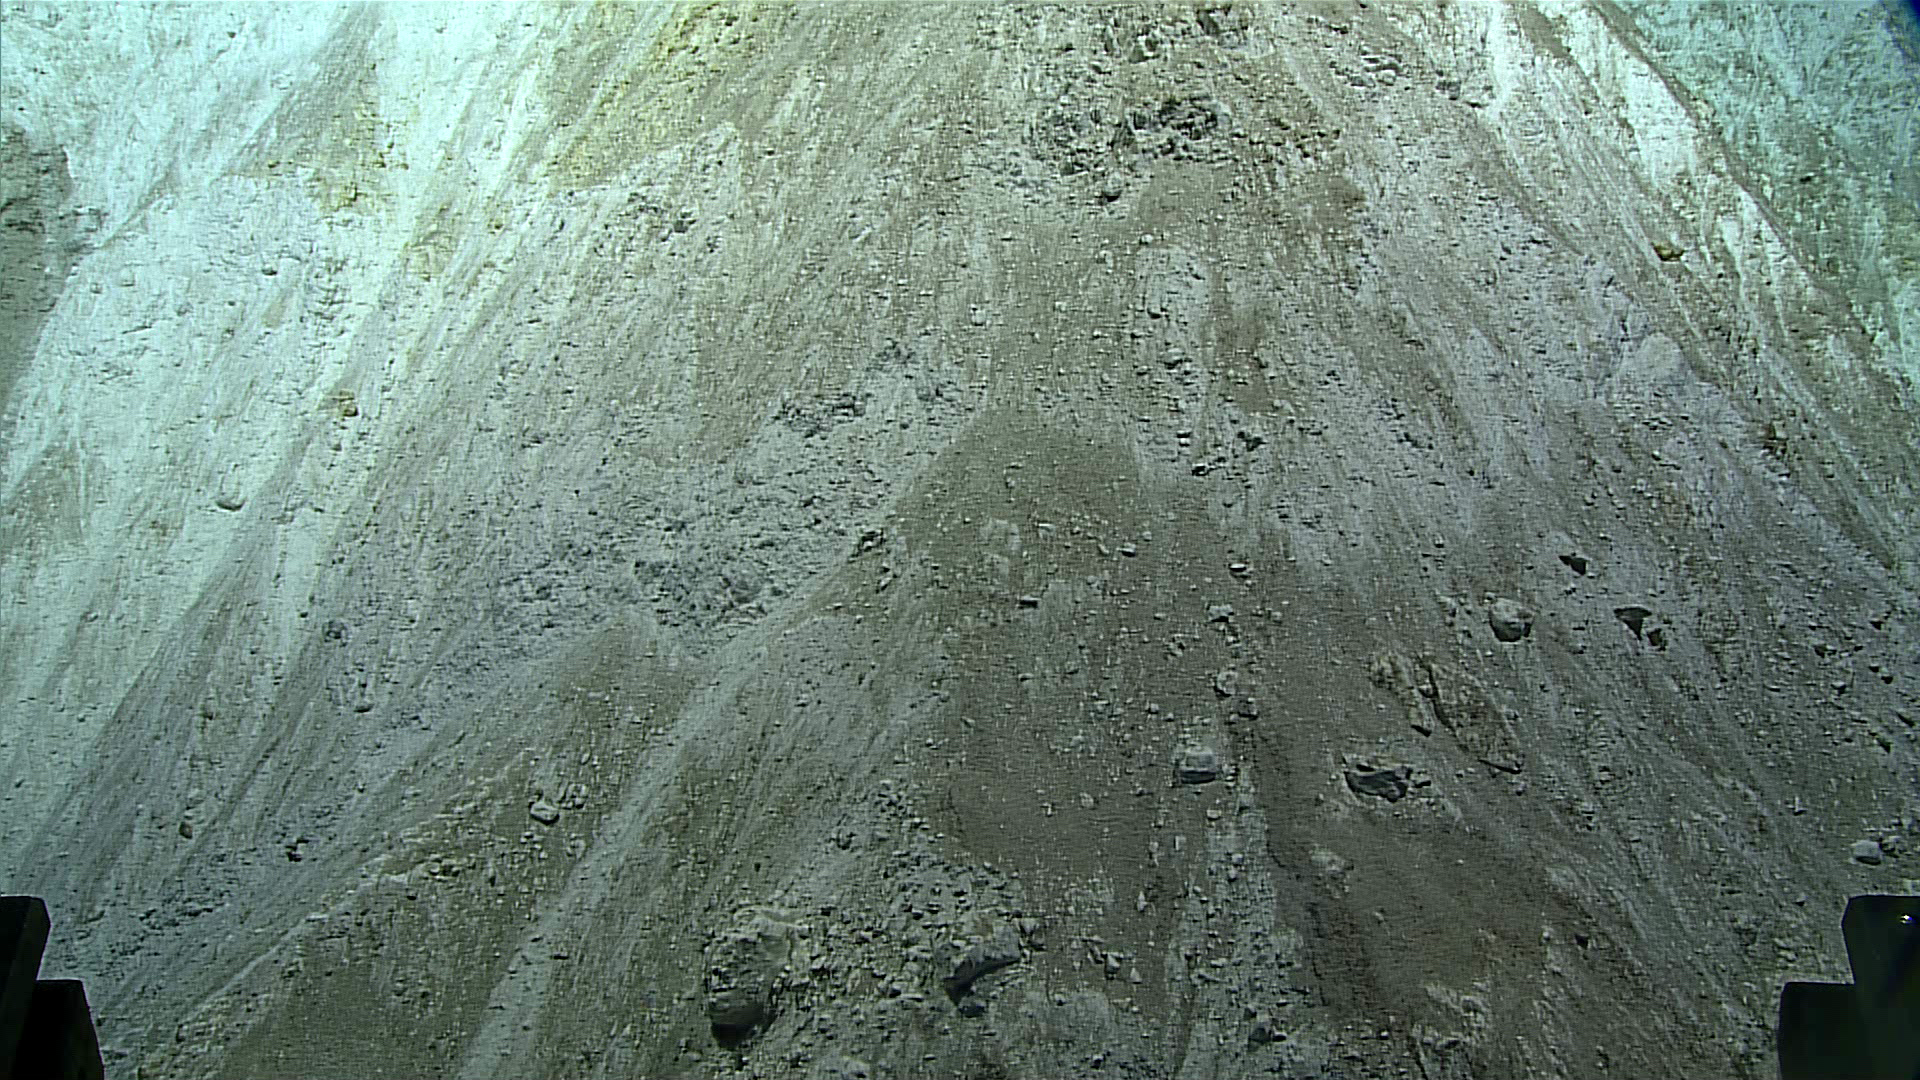
\includegraphics[width=\textwidth]{images/image_651100.png}
        \caption{Final frame in reconstructed segment, frame 651100 within dive.}
        \label{fig:ex1605l3_dive4_hillside_end}
    \end{subfigure}
    \caption{Source images for ``hillside'' reconstruction within dive EX1605L3\_DIVE4.}
\end{figure}

\begin{figure}
    \centering
    \begin{subfigure}[b]{0.48\textwidth}
        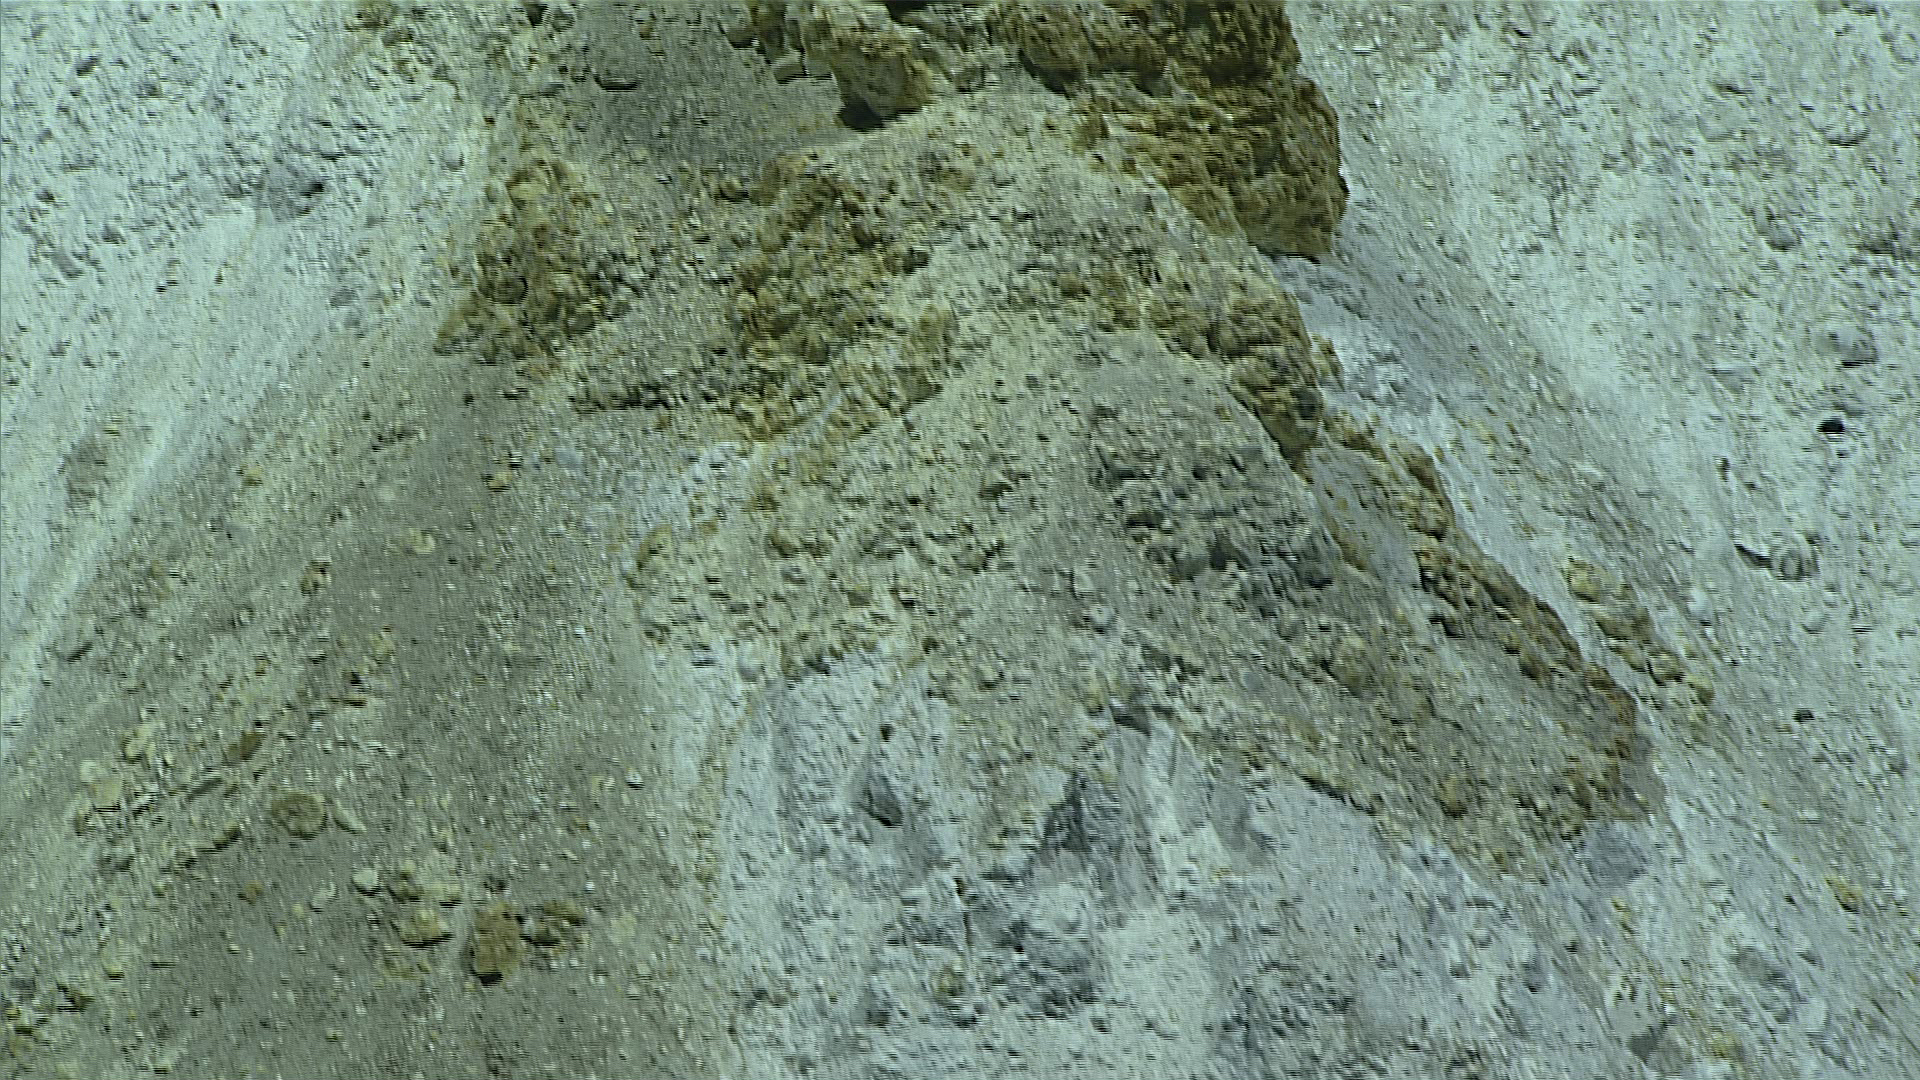
\includegraphics[width=\textwidth]{images/image_653000.png}
        \caption{First frame in reconstructed segment, frame 653000 within dive.}
        \label{fig:ex1605l3_dive4_upslope_begin}
    \end{subfigure}
    \begin{subfigure}[b]{0.48\textwidth}
        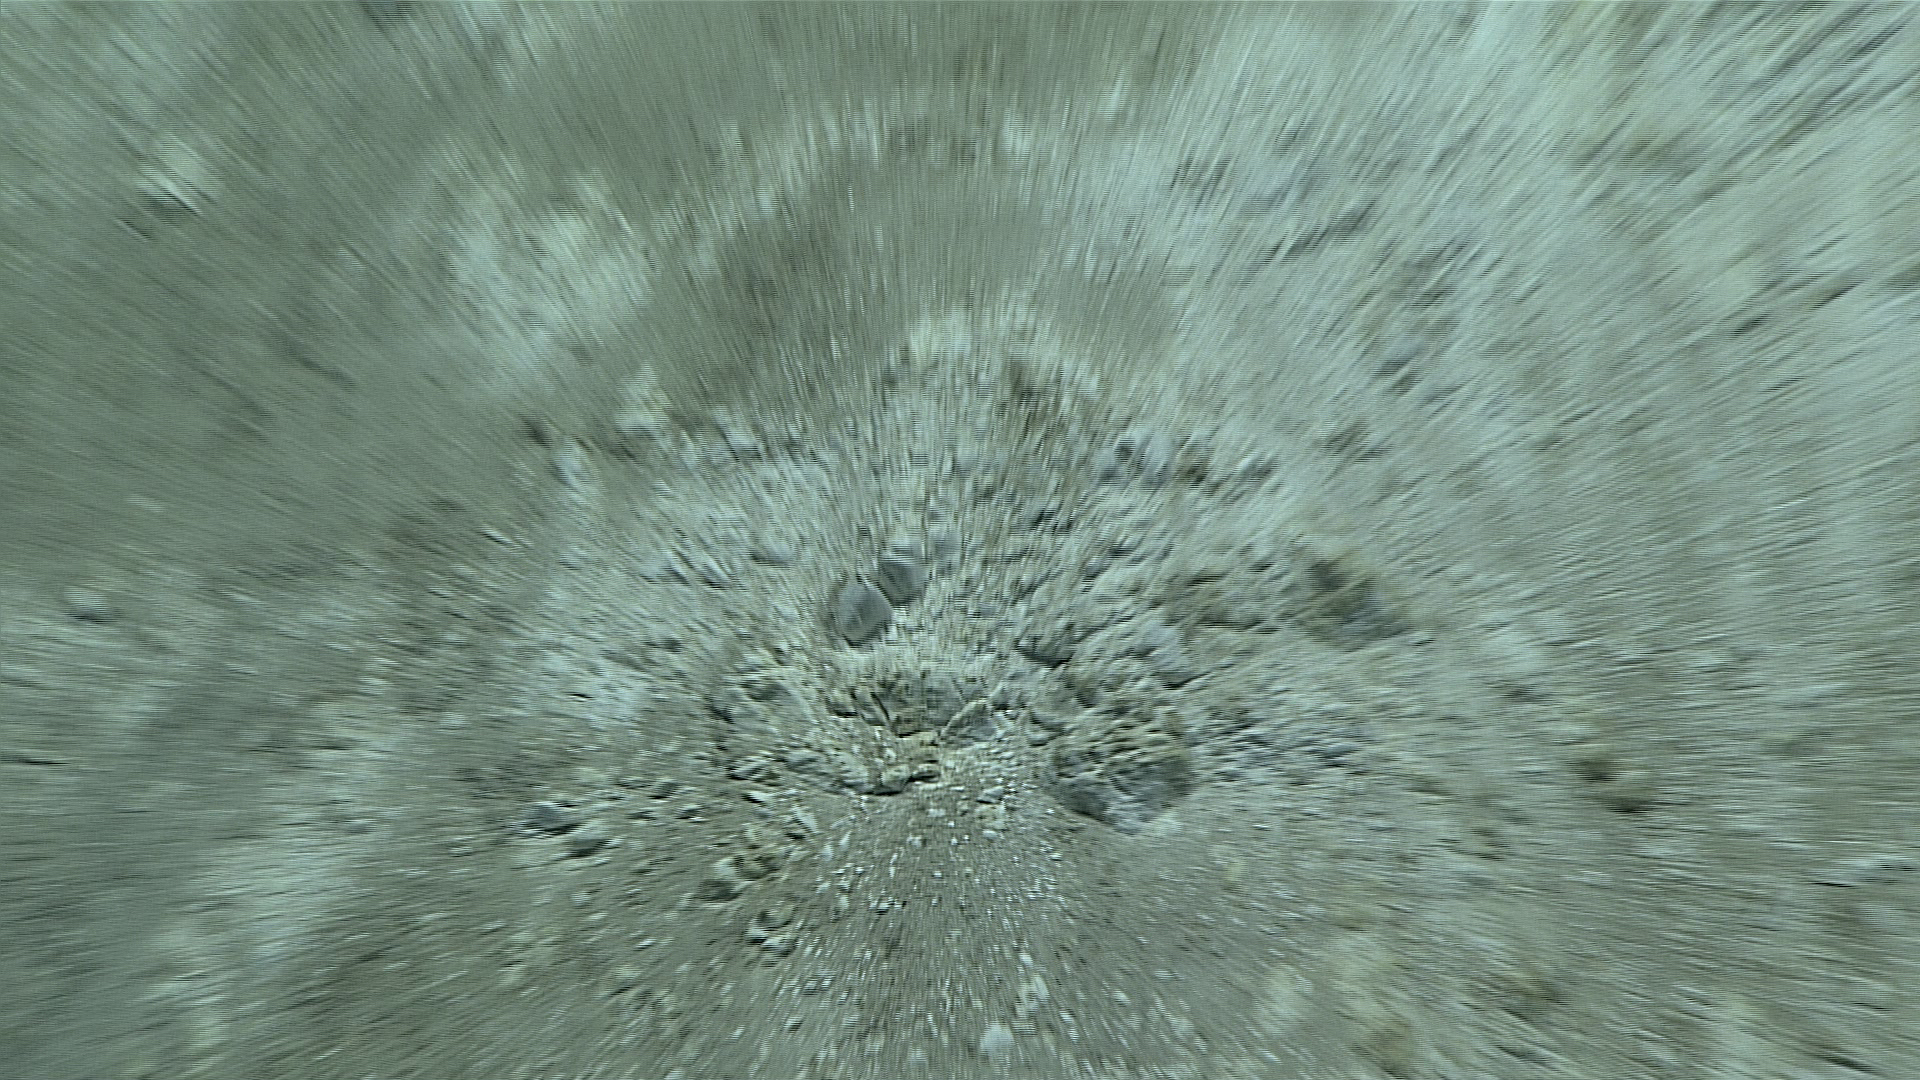
\includegraphics[width=\textwidth]{images/image_656500.png}
        \caption{Final frame in reconstructed segment, frame 656500 within dive.}
        \label{fig:ex1605l3_dive4_upslope_end}
    \end{subfigure}
    \caption{Source images for ``upslope'' reconstruction within dive EX1605L3\_DIVE4.}
\end{figure}

\begin{figure}
    \centering
    \begin{subfigure}[b]{0.48\textwidth}
        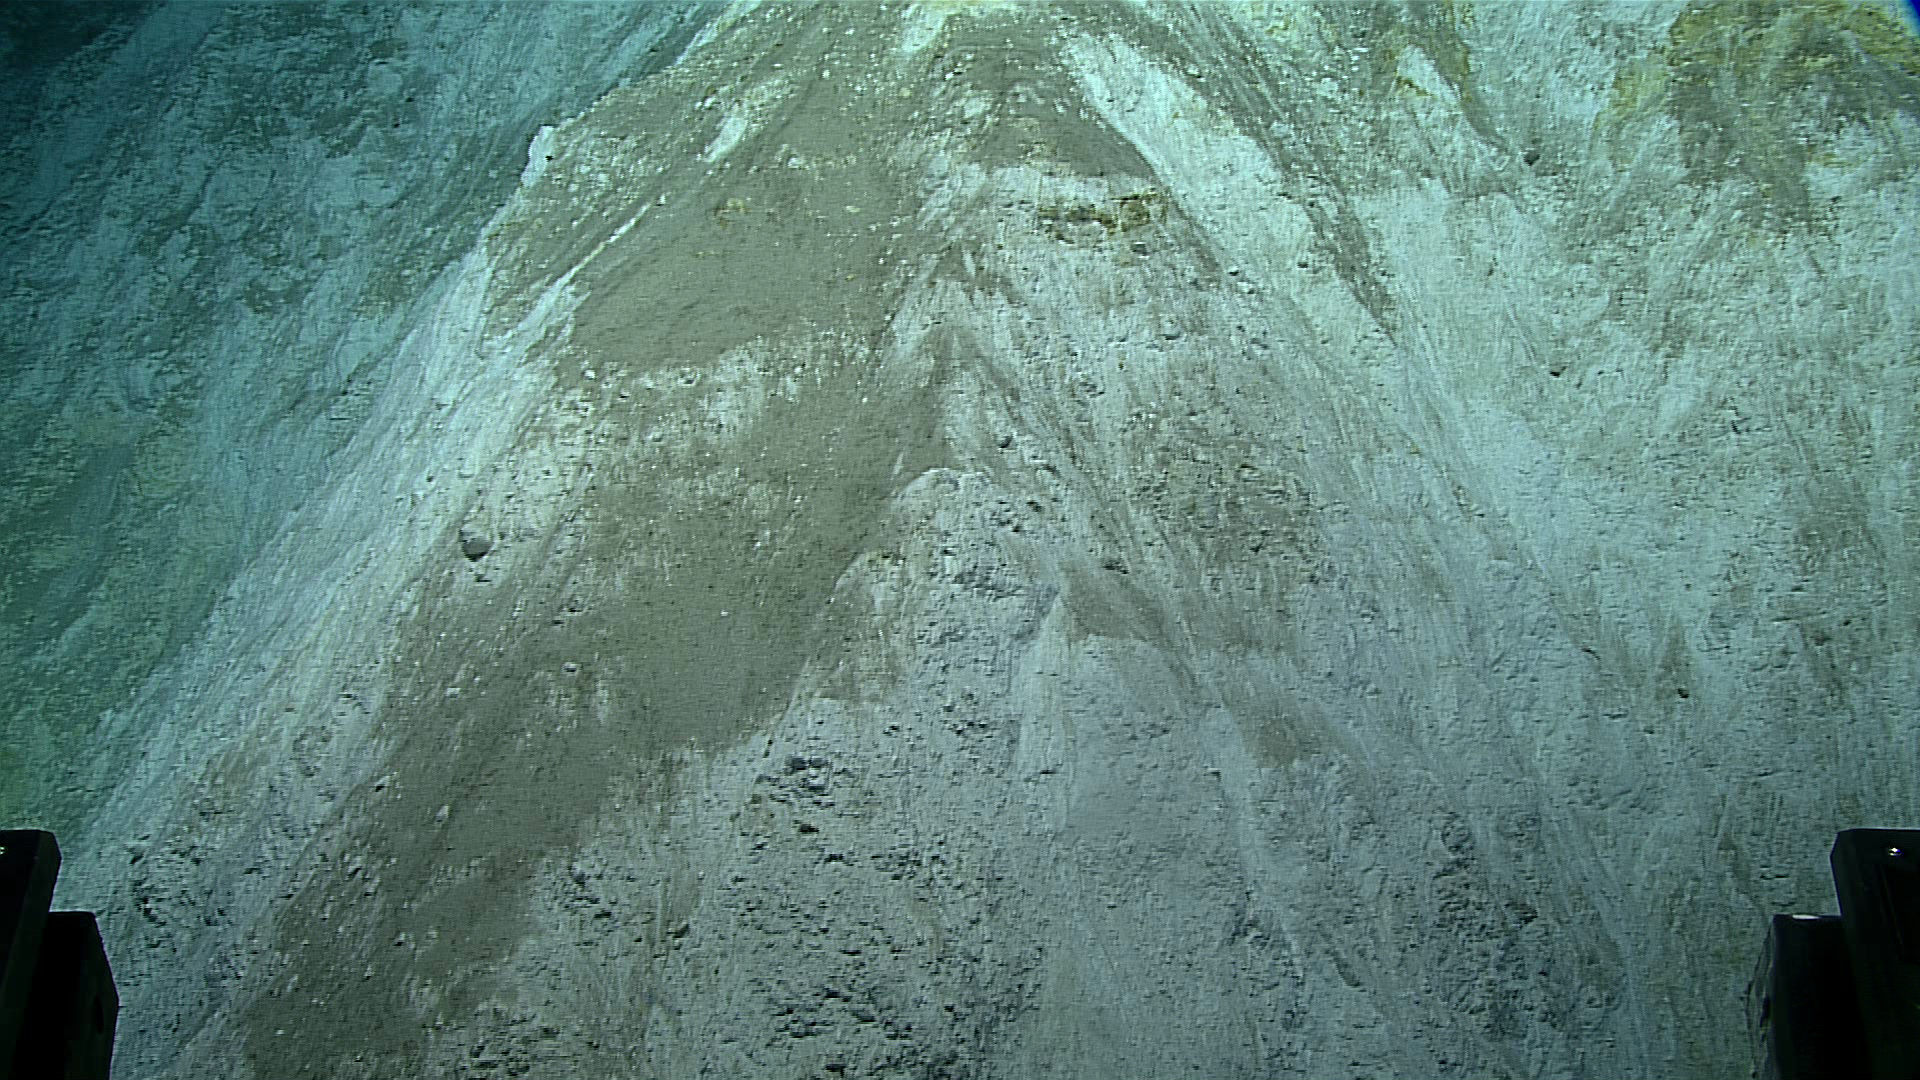
\includegraphics[width=\textwidth]{images/image_656700.png}
        \caption{First frame in reconstructed segment, frame 656700 within dive.}
        \label{fig:ex1605l3_dive4_top_of_slope_begin}
    \end{subfigure}
    \begin{subfigure}[b]{0.48\textwidth}
        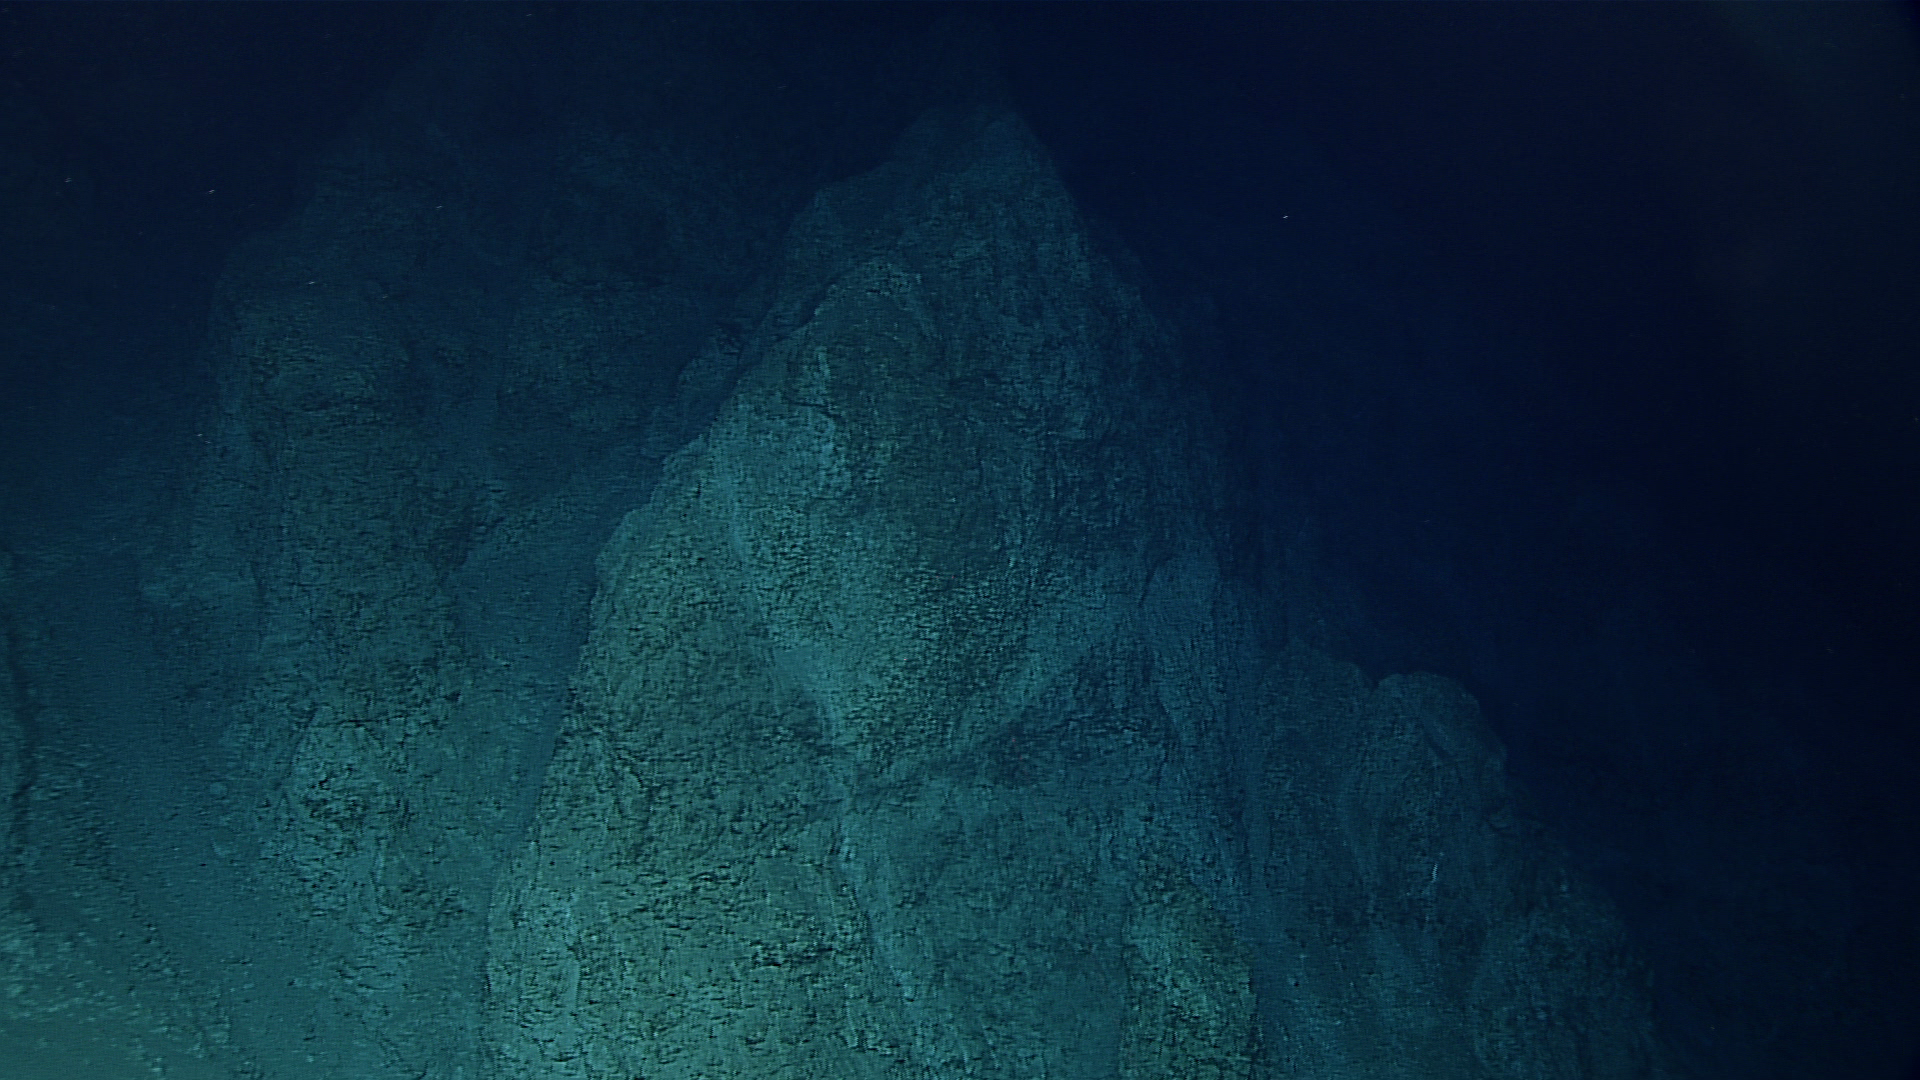
\includegraphics[width=\textwidth]{images/image_679900.png}
        \caption{Final frame in reconstructed segment, frame 679900 within dive.}
        \label{fig:ex1605l3_dive4_top_of_slope_end}
    \end{subfigure}
    \caption{Source images for ``top\_of\_slope'' reconstruction within dive EX1605L3\_DIVE4.}
\end{figure}

At the conclusion of ``hillside'', the main science camera zooms in partially and the ROV begins an upslope excursion, which is designated ``upslope''.  At the conclusion of this transit it then zooms back out and the ROV continues to maneuver further upslope over multiple ridges.  At the conclusion of this section, the ROV moves into open water and the seafloor is no longer visible (figure \ref{fig:ex1605l3_dive4_top_of_slope_end}).

A total of 82 images were extracted from ``hillside.'' and were successfully reconstructed in Photoscan (figures \ref{fig:ex1605l3_dive4_photoscan} and \ref{fig:ex1605l3_dive4_photoscan_trajectory}).  Figure \ref{fig:ex1605l3_dive4_photoscan_trajectory} shows the estimated trajectory of the camera (ROV) as estimated from the imagery.  This estimated trajectory is qualitatively correct, showing the ROV approaching the hillside (as bottom of image), then transiting (swaying) rightward across a valley to another ridge.   

\begin{figure}
    \centering
    \begin{subfigure}[b]{0.9\textwidth}
        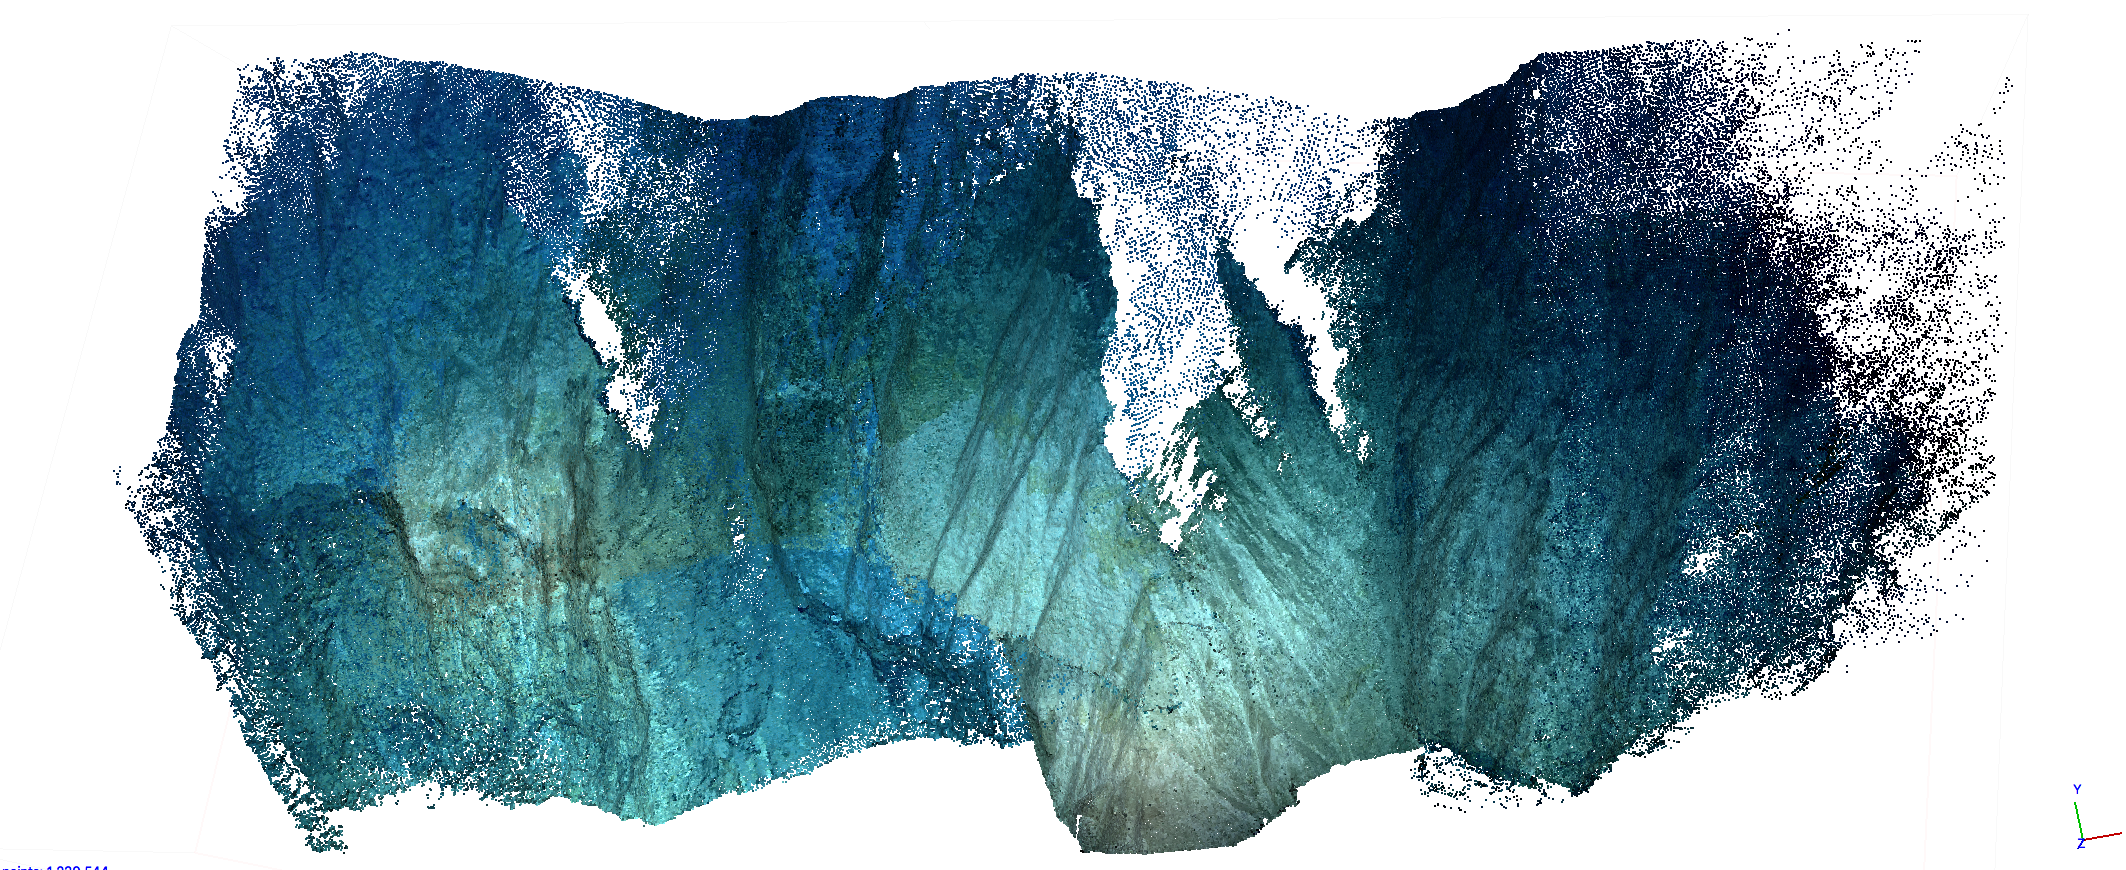
\includegraphics[width=\textwidth]{images/hillside_reconstruction.png}
        \caption{Dense point cloud from reconstruction of ``hillside'' video segment.}
        \label{fig:ex1605l3_dive4_photoscan}
    \end{subfigure}
    \begin{subfigure}[b]{0.9\textwidth}
        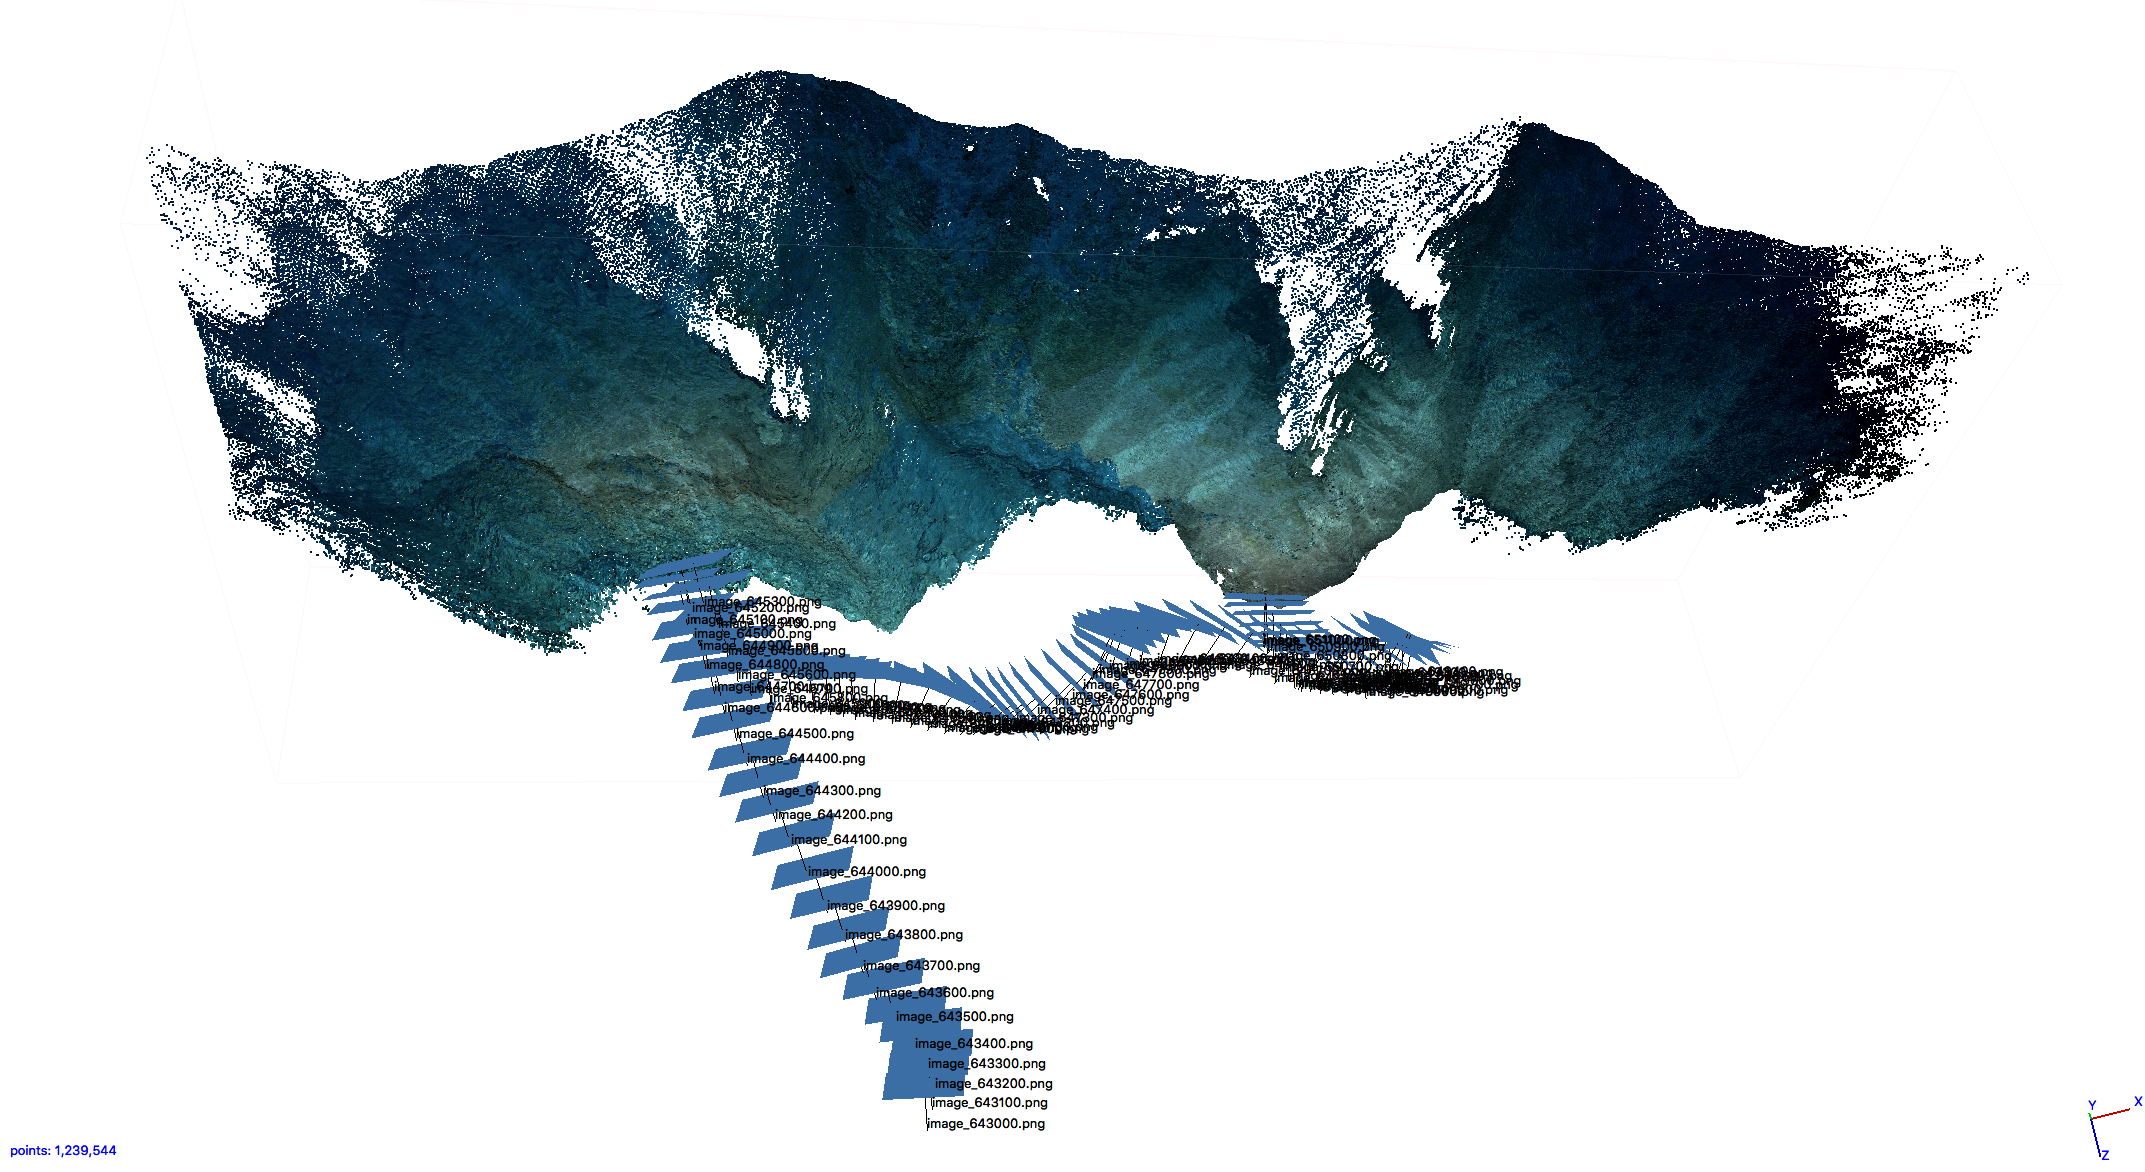
\includegraphics[width=\textwidth]{images/hillside_reconstruction_trajectory.png}
        \caption{Reconstruction with camera trajectory (shown as purple squares) overlaid.  Top edge of model has been pitched towards observer relative to figure \ref{fig:ex1605l3_dive4_photoscan}. }
        \label{fig:ex1605l3_dive4_photoscan_trajectory}
    \end{subfigure}
    \caption{Source images for ``top\_of\_slope'' reconstruction within dive EX1605L3\_DIVE4.}
\end{figure}

While qualitatively successful, this reconstruction illustrates many of the issues observed while reconstructing the ROV video.    Water quality taken at depth (approx. 6000m in this case) is very good, with little turbidity, however, the strong absorption of light creates an unmodelled --- and unique --- distortion in imagery.   In standard terrestrial imagery, the scene is generally evenly lit, often by natural light.   In this case, there is generally no dependency between the ``quality'' of the imagery of a given object and its distance from the camera, and instead the performance of reconstruction is a function solely of camera resolution.   In the ROV video, where the only light is mounted near the camera, distant objects undergo a fading in color and contrast well before they become too small to resolve.   For example, in ``hillside,'' the hillside is initially far from the ROV and is primarily blue-black in color (as in figure \ref{fig:ex1605l3_dive4_hillside_begin}).  As the ROV approaches, the optical path through the water decreases and the apparent color of the slope becomes the ``true'' brown-grey.   Despite this shifting appearance, Photoscan is able to complete reconstruction (in part because image matching algorithms work in greyscale), however, the impact of this color shifting can be seen in the mottled appearance of Figure \ref{fig:ex1605l3_dive4_photoscan}. 
Portions of the scene which are only seen from a distance (e.g., the upper and lower left)









Within dive 



\subsubsection*{Describe how the project was organized and managed}

All project work was performed and managed by the PI at UW-APL

\subsubsection*{Describe how data was organized, processed, and archived}

The source D2 data was provided by NOAA as full sets of Apple Quicktime / ProRes video files for each of four dives of interest, from surface to surface.   The files are split into 5 minute segements, and total approximately 4.2 TB for all four dives.   Data was delivered via an external hard drive and was subsequently stored in its original directory structure on a network attached drive at UW-APL.  Every effort was made to maintain the original data in its original format rather than perform extensive reorganization on the original raw video data.

\subsection{Findings}
\subsubsection*{Describe actual accomplishments and findings}


% \subsubsection*{Inventory of activities (number of submersible dives, CTD, net tows, etc.)}

% \subsubsection*{Inventory of samples collected}

\subsubsection*{Describe/list/append resulting publications, Web sites, presentations, etc.}

% Project progress is documented at the website \url{https://noaa-oer16-3dreconstruction.github.io/public-www/}.

A description of project outcomes is being prepared for the 2019 IEEE/MTS Oceans conference to be held in Seattle in October 2019.

\subsubsection*{Location and status of data archive and/or sample storage, plan for public access, and final data inventory} 



\subsubsection*{Notation of major changes/adjustments to previously submitted documents (e.g.    Quick Look Report, Semi-Annual Report, and/or Annual Report)}

\section{Evaluation}

\subsection{Accomplishments}

– Explain special problems, differences between scheduled and accomplished work

\subsection{Expenditures}

The award and final budget expenditures are detailed below:

\begin{tabularx}{0.9\textwidth}{X|rrrr}
    & \textbf{Award} & \textbf{Expenditures} & \textbf{Expenditures} &  \\
    & \textbf{Amount} & \textbf{Year 1} & \textbf{Year 2} & \textbf{Balance} \\
    \hline\hline
    Salaries \& Wages & \$36,122.00 & \$36,653.27 & \$4,528.01 & (\$5,059.28) \\
    Staff Benefits & \$18,685.00 & \$19,718.06 & \$2,763.35 & (\$3,796.41) \\
    Travel & \$11,496.00 & \$251.83 & --- & \$11,244.17 \\
    Services & --- & --- & --- & --- \\
    Supplies & \$1,000.00 & \$1,241.86 & \$370.02 & (\$611.88) \\
    Equipment & --- & --- & --- & --- \\
    Other & \$21,537.00 & \$20,346.25 & \$2,436.36 & (\$1,245.61) \\
    Indirect Cost & \$16,880.00 & \$14,860.13 & \$1,918.57 & \$101.30 \\
     \\
    Total & \$105,720.00 & \$93,071.40 & \$12,016.31 & \$632.29 
\end{tabularx}

\vskip{12pt}
\noindent
As per the original award, the project expenditures were almost exclusively salary support for the project team.  The original proposal included a trip to rendezvous with the D2 at a port of call to perform an explicit calibration of the main science camera.  This proved to be both challenging to schedule and unnecessary as the intrinsic properties of the camera could be derived directly from the data.

\subsection{Next Steps}
\subsubsection*{Planned or expected reports (professional papers, presentations, etc.)}
\subsubsection*{Brief description of need for additional work, if any (next project phase, new research questions, unaccomplished work, etc.)}

\bibliography{sample}






% \section{Problem and hypothesis} \label{sec:intro}
% Start your main text here.
% Add more sections as needed.
% In the first section of a paper it is appropriate to describe the area of research, the research problem to be solved and why it is important, the hypothesis and the expected outcome.

% Provide examples when appropriate.
% Examples (\ref{ex:dutch}) and (\ref{ex:norwegian}) illustrate the inclusion of lines with glosses.
% Figure \ref{fig:tree} illustrates how a tree structure can be drawn.

% \begin{exe}
% \ex \label{ex:dutch}
% \gll Dit is een Nederlands voorbeeld-je.\\
% This is a Dutch example-DIM\\
% \trans `This is a small example in Dutch.'

% \ex \label{ex:norwegian}
% \gll Dette er det norske eksemplet.\\
% This is the Norwegian example.DEF\\
% \trans ‘This is the Norwegian example.’
% \end{exe}

% \begin{figure}[htbp] \begin{center}
% \synttree [S [NP [Pro [He]]] [VP [V [died]] [PP [P [for]] [NP [Pro [her]]]]]]
% \caption{An example tree drawn from labeled bracketing using the \emph{synttree} package.} \label{fig:tree}
% \end{center} \end{figure}

% \section{Data and Method}
% It is often appropriate to devote a section to the description of the data and the method used.
% This section could, for instance, describe corpus materials, lexical data, questionnaires, machine learning programs, or other data sources, methods and tools which you have used for your paper.
% Be specific.
% If you search in a corpus, for instance, specify which corpus was consulted on which site, and give your exact search expressions.
% Provide datasets, questionnaires or other materials in the appendices if they are larger than about a page.
% Materials spanning more than five pages or encoded in other ways than plain text should preferably not be included in the PDF, but can be put in a ZIP or RAR archive together with the main file.

% Include relevant references to related work \citep{Van-Dongen12}.
% References to web resources\footnote{Wikibooks: \url{http://en.wikibooks.org/wiki/LaTeX}} can also be put in footnotes.
 
% \section{Results}
% This section could describe the results obtained from the research.
% Present quantitative results in tables and/or graphs, as illustrated in Table \ref{tab:freq} and Figure \ref{fig:proportion}.

% \input{boysgirlsnormtable}

% \begin{figure}[htb] \begin{center}
% \includegraphics[width=0.7\textwidth]{boysgirls}
% \caption{Normalized frequencies, pairwise} \label{fig:proportion}
% \end{center} \end{figure}

% \section{Discussion and conclusion}
% The last section normally attempts to interpret the results and investigates if the results confirm or reject the initial hypothesis formulated in section \ref{sec:intro}.
% The conclusion summarizes which new knowledge is obtained, and possibly what it can be used for.
% It also discusses to what extent the outcomes are uncertain or of a limited scope.



% \appendix
% \section{Frequency list exclusive of hapax legomena} \label{app:freq}
% This is an example appendix showing how raw data can be included from a separate file.

% \begin{multicols}{3}
% {\footnotesize\verbatiminput{askefreqnohapax}}
% \end{multicols}

% \section{Reflection notes} \label{app:reflection}
% \emph{This section is obligatory for DASP307 only.}
% Write some notes about your intended audience, the role of the paper in your study program, strategies for communicating with the reader and for citing other work, rhetorical strategies to convince the reader, motivation for your use of examples, figures, tables, etc.
\end{document}